% Template for PLoS
% Version 1.0 January 2009
%
% To compile to pdf, run:
% latex plos.template
% bibtex plos.template
% latex plos.template
% latex plos.template
% dvipdf plos.template

\documentclass[11pt]{article}

% amsmath package, useful for mathematical formulas
\usepackage{amsmath}
%\usepackage{natbib}
% amssymb package, useful for mathematical symbols
\usepackage{amssymb}
\usepackage{booktabs}
\usepackage{xspace}
% graphicx package, useful for including eps and pdf graphics
% include graphics with the command \includegraphics
\usepackage{graphicx}


% cite package, to clean up citations in the main text. Do not remove.
\usepackage{cite}
\usepackage{caption}
\usepackage{subcaption}

\usepackage{color} 

% Use doublespacing - comment out for single spacing
%\usepackage{setspace} 
%\doublespacing


% Text layout
\topmargin 0.0cm
\oddsidemargin 0.5cm
\evensidemargin 0.5cm
\textwidth 16cm 
\textheight 21cm

% Bold the 'Figure #' in the caption and separate it with a period
% Captions will be left justified
\usepackage[labelfont=bf,labelsep=period,justification=raggedright]{caption}

% Use the PLoS provided bibtex style
\bibliographystyle{/Users/stephens/Dropbox/Documents/stylefiles/plos2009}

% Remove brackets from numbering in List of References
\makeatletter
\renewcommand{\@biblabel}[1]{\quad#1.}
\makeatother


% Leave date blank
\date{}

\pagestyle{myheadings}
%% ** EDIT HERE **
\usepackage{enumerate}
\usepackage{multirow} 
\usepackage{url}
\usepackage{xr} %for cross-referencing
%% ** EDIT HERE **
%% PLEASE INCLUDE ALL MACROS BELOW
\newtheorem{algorithm}{Algorithm}
\newtheorem{proposition}{Proposition}
\newtheorem{restateproposition}{Proposition}
\newtheorem{lemma}{Lemma}
\newtheorem{corollary}{Corollary}
\newtheorem{result}{Result}
\newtheorem{note}{Note}
\newtheorem{definition}{Definition}

\def\lfdr{\text{lfdr}}
\def\lfsr{\text{lfsr}}
\def\x{\mbf{x}}
\def\y{\mbf{y}}
\def\e{\mbf{e}}
\def\g{\mbf{g}}
\def\p{p}
\def\Yb{\hat{Y}_1^{\text{BAYES}}}
\def\Xperp{X_{1 \perp 0}}
\def\Pperp{P_{1 \perp 0}}
\def\Pperpb{\Pperp^{\text{B}}}
\def \hatd { \widehat{ d } }
\def \dhatin {\hatd^{\mbox{\tiny IN}}}
\def \dhatsw {\hatd^{\mbox{\tiny SW}}}
\def \mvn{\text{MVN}}
\def\mn{\text{MN}}
\def \iw{\text{W}^{-1}}
\def \fp {fastPHASE\ }
\def\bhat{\hat{\beta}}
\def\shat{\hat{s}}
\def\var{\rm Var}
\def\mvr{\text{BMVR}}
\def\bfuni{\text{BF}_\text{uni}}
\def\one{\mbf{1}}
\def\zero{\mbf{0}}
\def\hall{H_{\text{all}}}
\def\pall{\p_{\text{all}}}
\def\bfall{\text{BF}_\text{all}}
\def\bfav{\text{BF}_\text{av}}
\def\gall{\gamma_\text{all}}
\def\limbfall{\bfall^\rightarrow}
\def\limbfav{\bfav^\rightarrow}
\def\limbfgamma{\BF_\gamma^\rightarrow}
\def\sxx{S_{xx}}
\def\syy{S_{yy}}
\def\vyy{V_{yy}}
\def\vyx{V_{yx}}
\def\vxx{{V_{xx}}}
\def\rss{\text{\rm RSS}}
\def\dss{\text{\rm $\Delta$SS}}
\def\U{U}
\def\D{D}
\def\I{I}
\def\luu{L_{UU}}
\def\indep{\perp}
\def\qvalue{{\tt qvalue}\xspace}
\def\locfdr{{\tt locfdr}\xspace}
\def\mixfdr{{\tt mixfdr}\xspace}
\def\ashr{{\tt ashr}\xspace}

\newcommand{\mbf}[1]{\mbox{\boldmath$#1$}} % true mathbf works in math
                                % mode too
\newcommand\height{{\it height}}
\newcommand\weight{{\it weight}}
\def\BF{\text{BF}}


%% END MACROS SECTION
%\externaldocument{plos_one_rev1_suppinfo}

\begin{document}

% Title must be 150 characters or less
\begin{flushleft}
{\Large
\textbf{False Discovery Rates: A New Deal}
}
% Insert Author names, affiliations and corresponding author email.
\\
Matthew Stephens$^{1*}$, 
\\
\bf{1} Department of Statistics and Department of Human Genetics, University of Chicago, Chicago, IL, USA
\\
$\ast$ E-mail: Corresponding mstephens@uchicago.edu
\end{flushleft}

% Please keep the abstract between 250 and 300 words
\section*{Abstract}

% Please keep the Author Summary between 150 and 200 words
% Use first person. PLoS ONE authors please skip this step. 
% Author Summary not valid for PLoS ONE submissions.   
%\section*{Author Summary}

\section*{Introduction}

Since its introduction in 1995 by Benjamini and Hochberg 
\cite{benjamini1995controlling}, the ``False Discovery Rate" (FDR) has quickly established itself
as a key concept in modern statistics, and the primary tool by which most practitioners handle large-scale multiple testing
in which the goal is to identify the non-zero ``effects" among a large number of imprecisely-measured effects.

Here we consider an Empirical Bayes (EB) approach to FDR. This idea is, of course, far from new:
indeed, the notion that EB approaches could be helpful in handling multiple comparisons predates introduction of
the FDR  (e.g.~\cite{greenland1991empirical}). More recently, EB approaches to the FDR
have been extensively studied by several authors, 
especially B.~Efron and co-authors 
\cite{efron2001empirical, efron2002empirical,efron2003robbins,efron2008microarrays,efron2010large}; 
see also \cite{kendziorski2003parametric,newton2004detecting, 
datta2005empirical,muralidharan2010empirical} for example.
So what is the ``New Deal" here? We introduce two simple ideas that are new (at least compared with
existing widely-used FDR pipelines) and can substantially improve
inference. The first idea is to {\it assume that the distribution of effects is unimodal}, and to perform
non-parametric inference under this assumption. This idea leads to a very simple, fast, and stable computer implementation,
 and improves inference of FDR, at least when the unimodal assumption is correct. 
 (And when the assumption is incorrect, errors in inference are not too egregious.) 
The second idea is to use two numbers -- effect sizes, and their standard errors -- rather than just one -- $p$ values, or $z$ scores -- 
to summarize each measurement. This idea allows variations in measurement precision to be accounted for,
 and avoids the problem with standard pipelines that poor-precision measurements can inflate estimated FDR.

In addition to these two new ideas, we highlight a third idea that is old, but which remains under-used in practice:
the idea that it may be preferable to focus on estimation rather than on testing.
In principle, Bayesian approaches can naturally unify testing and estimation into a single framework -- testing is
simply estimation with some positive prior probability that the effect is exactly zero.
However, despite ongoing interest in this area from both frequentist \cite{benjamini2005false} and Bayesian \cite{zhao2012empirical,gelman2012we} 
perspectives, in practice large-scale studies that assess many effects almost invariably focus on testing significance and
controlling the FDR, and not on estimation. To help provide a bridge between FDR and estimation we introduce the terminology
``signed discovery" for a discovery (an effect declared to be non-zero) for which the sign of the effect (positive or negative) is declared,
and correspondingly define the ``false signed discovery rate" (FSDR) in a natural way. We show that in some settings, particularly those with many discoveries, 
the FSDR and FDR can be quite different, and emphasise benefits of the FSDR, particularly its increased robustness to modelling assumptions. 

%The methods we provide here can address both problems, and we provide results that highlight important benefits of focussing on estimation, and particularly on assessing the correctness of the {\it sign} of the estimated effects, rather than on testing for non-zero effects.


The use of EB methods for estimation also has a long and close relationship with another key concept in modern statistics: shrinkage estimation \cite{efron1973}.
This close relationship becomes especially intimate here due to our unimodal assumption on the underlying effects, 
which encourages shrinkage towards the mode of the distribution.
%Indeed, within our EB framework, multiple comparisons correction can be seen as a natural limit of shrinkage estimation:
%if effects are distributed uni-modally about zero then it is natural to shrink estimates towards zero. 
% are essentially two sides of the same coin, one related to testing and the other to estimation. 
Thus, although we focus here primarily on FDR-related issues, another important contribution of our work is to provide {\it generic} and {\it adaptive} shrinkage estimation procedures.
By generic, we mean that these methods can be applied in any setting where a series of effect estimates and corresponding standard errors are available.
By adaptive, we 
have two properties in mind. First, the appropriate amount of shrinkage is determined from the data: when the data indicate that large effects are relatively common then
shrinkage of large observed effects is less than when the data indicate that large effects are rare.
Second, the amount of shrinkage undergone by each measurement will depend on its precision, or standard error: measurements with big standard errors undergo more shrinkage than measurements with small standard errors.  
Shrinkage estimation is a powerful tool, with many potential applications, including for example wavelet denoising, 
where shrinkage of wavelet coefficients is used to smooth signals. Our methods provide an attractive and competitive alternative
to existing EB shrinkage methods for that context, as will be explored more fully elsewhere (Xing and Stephens, in preparation).

Our methods are implemented in an R package, \ashr (for {\bf a}daptive {\bf sh}rinkage in {\bf R}), available at \url{http://github.com/stephens999/ashr}.



%Measurement precision will often vary among genes --  for example, log-fold change estimate for highly expressed genes may have greater precision than those for lower-expressed genes -- and one goal  of our methods is to allow for thiis variation. 

%Let $\mu^0_j$ and $\mu^1_j$ denote the mean expression 
%of gene $j$ ($j=1,\dots,J$) in the two conditions, and define $\beta_j:= \mu^0_j - \mu^1_j$ to be the difference. Typically expression
%measurements are made on only a small number of
%samples in each condition - sometimes as few as one
%sample in each condition. Thus the error in estimates
%of $\mu^0_j$ and $\mu^1_j$ is appreciable, and the error
%in estimates of $\beta_j$ still greater.
%

%Many tools have been developed for estimating or controlling the FDR and related quantities \cite{}, and some are widely used.
%Here we present new tools that bring two important ideas to bear on the problem.
%First, these tools are designed to take account of variations in the {\it measurement precision} of different effects, reducing the influence of low-precision measurements.
%For example, in the example of detecting differentially expressed genes, measurements of log fold change for high-expressed genes 
%may have better precision than those for low-expressed genes; by incorporating this information our methods can avoid the tendancy for 
%imprecise measurements at low-expressed genes to dilute the signal at higher-expressed genes.
%Second, our tools explicitly assume that the non-zero effects have a unimodal distribution centered at zero. This assumption 
%is, we argue, often realistic, and comes with considerable benefits, both statistical and computational. 
%Our tools are implemented in an R package \ashr (short for ``Adaptive Shrinkage") and we 
%demonstrate how the incorporation of these two ideas can lead to a substantial reduction in estimated FDRs (or, equivalently,
%a substantial increase in the number of discoveries at a given FDR).  

%Although we motivate our tools by the need to address the FDR problem, our \ashr package, as its name suggests,  provides a general tool for shrinkage estimation. 
%As an important special case, these methods address the "multiple comparisons" setting, where interest usually focuses on which $\beta_j$ can be confidently inferred to be non-zero. Such problems are usually tackled by computing a $p$ value for each $j$, often by applying a $t$ test to $\bhat_j/s_j$,
%and then applying a generic procedure, such as that of \cite{benjamini1995controlling} or \cite{storey2003statistical}, designed to control or
%estimate the false discovery rate (FDR) or the positive FDR \cite{storey.03}. In essence we aim to provide analagous
%generic methods that work directly with two numbers for each 
%measurement $(\bhat_j,s_j$), rather than a single number (e.g.~ the $p$ value, or $t$ statistic). Working with these two numbers has two important benefits: first, it permits estimation and not only testing; second, the 
%uncertainty in each measurement $\bhat_j$ can be more fully accounted for, reducing the impact of ``high-noise" measurements (large $s_j$) that can reduce the effectiveness of a standard FDR analysis. 

\def\df{df}
\def\FDR{\text{FDR}}
\def\fdr{\text{lfdr}}
\def\FSDR{\text{FSDR}}
\def\fsdr{\text{lfsdr}}

 \section*{Methods}
 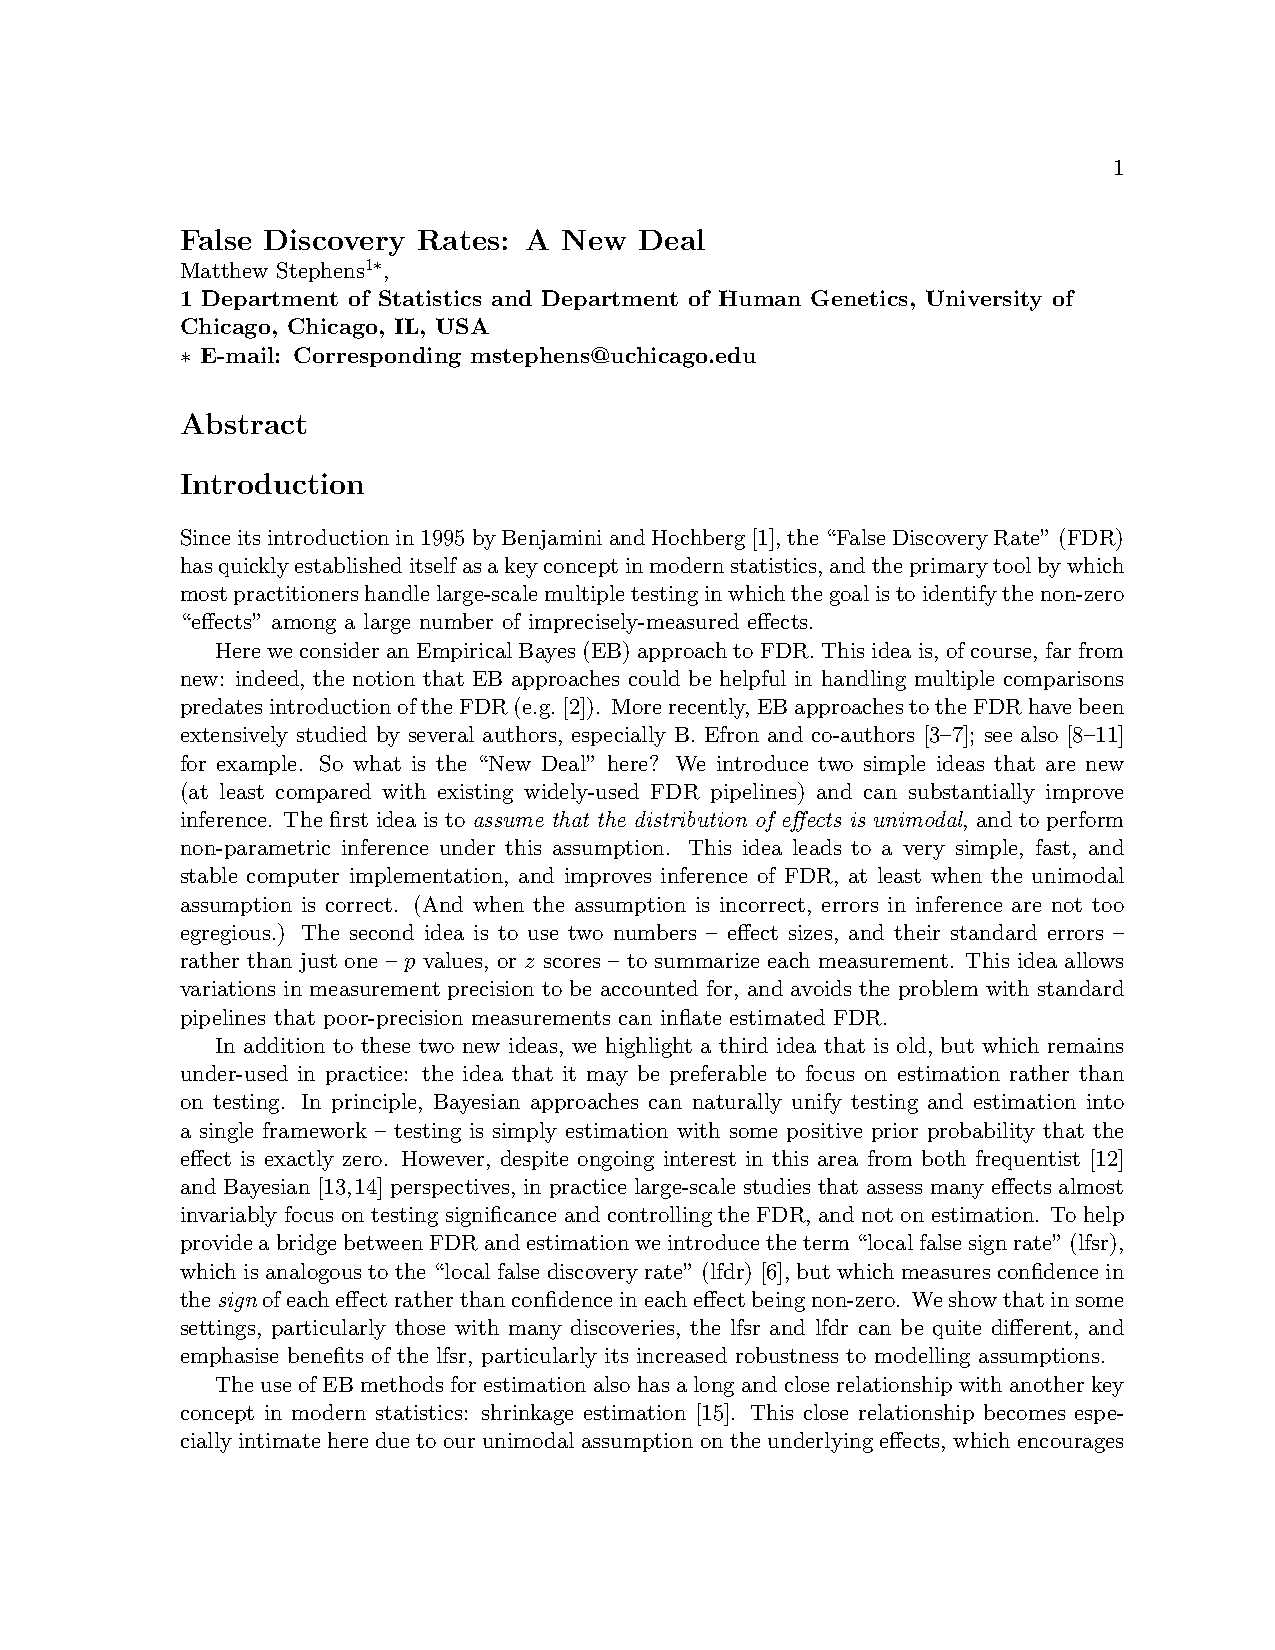
\includegraphics[]{main.pdf}

 \subsection*{Notation}
 
% Here we consider one setting in which FDR-based methods are widely used:
%an experimenter has measured a large numbers of ``effects", each with an associated
%measurement precision (standard error), 
%and the goal is to identify which of the effects we can declare to be non-zero, with some prescribed level of confidence.
%Although the usual focus of FDR-based methods is on distinguishing zero and non-zero effects,
%here we also focus on providing estimates -- both point estimates and interval estimates -- for these effects.
%This setting arises commonly in many areas of statistics, and particularly in genomics applications.
%For example, in genomics
%a common goal is to identify ``differentially-expressed genes" -- that is, genes
%whose mean expression (activity) level differs in two conditions. Here the ``effect" of interest is the difference in (log) 
%mean expression level between the two conditions, often referred to as the ``log-fold change". 

Suppose that we are interested in the values of $J$ ``effects" $\beta_j$ ($j=1,\dots,J$). For example, in a canonical genomics application
$\beta_j$ might be the difference in the mean (log) expression of gene $j$ in two conditions.
In some contexts interest may focus on which of the $\beta_j$ are ``significantly" different from zero, whereas in other contexts interest may focus on estimating their values; the methods described here tackle both these problems.
 We assume that we have obtained data $D$ that consist of estimates $\bhat_1,\dots,\bhat_J$ of these effects,
 with corresponding (estimated) standard errors $\shat_1,\dots,\shat_J$. Let $H_j$ denote the event that the $j$th null hypothesis holds ($H_j:\beta_j=0$), and $t_j$ denote
 the $t$ statistic testing this null:
 \begin{equation}  
 t_j :=\bhat_j/\shat_j. 
 \end{equation}
 The $t$ statistics, of course, have a $t$ distribution under the null:
 \begin{equation} \label{eqn:tstat}
 t_j | H_j \sim T_\nu
 \end{equation}
 where $T_\nu$ denotes the $t$ distribution on $\nu$ \df, with $\nu$ assumed known. 
 Let $p_j$ denote the $p$ value obtained by comparing $t_j$ with its null distribution,
 \begin{equation}
 p_j := \Pr(|T_\nu| > |t_j| ).
 \end{equation}
Some methods for FDR analysis require $z$ scores instead of $t$ statistics or $p$ values;
 these methods can be applied by translating each $t_j$ into a corresponding
$z$ score, which we denote $z_j$.


 %For our purposes, these estimates and standard errors could be obtained from the data
%using any method, provided they (approximately) satisfy 
% \begin{equation} \label{eqn:betahat-t}
% \bhat_j \big{|} \, \beta_j, \shat_j \sim t_\nu(\beta_j,\shat_j),
% \end{equation}
%for some known degrees of freedom (\df) $\nu$, where $t_\nu(\mu,\sigma)$ denotes the generalized $t$ distribution on $\nu$ \df, with mean $\mu$ and scale parameter $\sigma$. (Equivalently, $(\bhat_j-\beta_j)/\shat_j \big{|} \, \beta_j \sim t_\nu$, where $t_\nu$ denotes the standard $t$ distribution on $\nu$ \df.)
%In the special case $\nu \rightarrow \infty$ this includes the situation where the $\bhat$ can be considered normally distributed:
%  \begin{equation} \label{eqn:betahat-norm}
% \bhat_j  \big{|} \, \beta_j, \shat_j \sim N(\beta_j,\shat^2_j).
% \end{equation}
% Assuming (\ref{eqn:betahat-t}), the $t$-statistics defined by
 

Let $\Gamma$ denote a subset of the tests $1,\dots,J$ declared ``significant" by some procedure. 
We define the FDR for $\Gamma$ as the proportion of these tests that are ``false discoveries" in that $H_j$ is true:
\begin{equation} \label{eqn:FDR}
\FDR(\Gamma) := \frac{\#\{j: H_j \cap j \in \Gamma\}}{\#\{j: j \in \Gamma\}},
\end{equation}
taken to be 0 if both numerator and denominator are 0. Frequentist approaches to controlling the FDR attempt to control
the expectation of $\FDR(\Gamma)$ where the expecation is taken over the sampling distribution of $\Gamma$ (which is a function of the procedure
used, considered fixed, and the data $D$, considered random). Bayesian approaches, in contrast, condition on the observed data, and compute
the posterior distribution for the $H_j$ given the data, which induces a posterior distribution on $\FDR(\Gamma)$. This posterior
distribution can be used to obtain a point estimate for $\FDR(\Gamma)$, for example using the posterior mean. 
To be more explicit, Bayesian (and EB) approaches give the posterior probability that $H_j$ holds, which
analagous to \cite{efron2008microarrays} we refer to as the ``local FDR", and denote $\fdr_j$:
%\begin{equation} \label{eqn:FDR}
%\FDR(T) := \Pr(\text{$H_j$ false} | t_j \geq T).
%\end{equation}
\begin{equation} \label{eqn:fdr}
\fdr_j := \Pr(H_j | D).
\end{equation}
The FDR can be estimated by the posterior mean for $\FDR(\Gamma)$, given by
\begin{equation} 
\widehat\FDR(\Gamma) := \frac{\sum_{j \in \Gamma} \fdr_j }{\#\{j: j \in \Gamma\}}.
\end{equation}
Although our approach here is (Empirical) Bayesian, one nice feature of FDR procedures is that 
Frequentist and Bayesian procedures are often closely aligned, at least under certain assumptions; see
for example \cite{storey.03}, particularly his Theorem 1. 


The $q$ value for observation $j$ is defined \cite{storey.03} as, roughly, the FDR for the set of observations that are at least as significant as observation $j$.
In a Bayesian analysis it is natural to order the significance of the hypotheses by $\fdr_j$, so we define
\begin{equation}
q_j := \widehat\FDR(\{k:\fdr_k \leq \fdr_j\}).
\end{equation}
%In simple settings (e.g. symmetric effects, with the same standard error) $\fdr_j$ is a monotonic function of the $p$ value $p_j$, and so
%\begin{equation}
%q_j = \widehat\FDR(\{k:p_k \leq p_j\})
%\end{equation}
%which is close to the definition in \cite{storey.03}.

\subsection*{The local False Sign Rate}

\cite{gelman2012we} emphasise that there are settings where
$\beta_j=0$ is implausible, in which case the FDR is not useful: if every $\beta_j$ is non-zero then there
is no such thing as a false discovery and the FDR will always be identically 0. 
Gelman et.~al.~suggest that in such settings we should replace the concept of a false discovery with the
concept of an ``error in sign". The idea is that, in settings where $\beta_j=0$ is implausible, the most fundamental
inference objective is to ask which $\beta_j$ are positive and which are negative.
Indeed, even in settings where some
$\beta_j$ are exactly zero, separately identifying which are positive and which negative may be useful. For example, when identifying differentially expressed genes,
analysts will often separate the genes that are ``upregulated" from those that ``downregulated" in a condition.
Further, this idea has a long history: for example, \cite{tukey1962future}, p32, suggests one should address
\begin{quote}
...the more meaningful question: ``is the evidence strong enough to support a belief that the observed difference has the correct sign?"
\end{quote}

Motivated by this, we define the local False Sign Rate (lfsr) for observation $j$ as 
\begin{equation}
\lfsr_j := \min[ p(\beta_j \geq 0| \bhat, s), p(\beta_j \leq 0| \hat\pi, \bhat, s) ].
\end{equation}
Thus $\lfsr_j$ gives the probability that we would get the sign of $\beta_j$ wrong if we
were to make our best guess. (Naturally, we consider it an error to state that $\beta$ is positive or negative when it is truly zero.)
To illustrate, suppose for concreteness
that the minimum is achieved by the first term, $p(\beta_j \geq 0| \bhat, s)=0.05$ say. Then
our best guess would be that $\beta$ is negative, and the probability that we have
made an error in sign would be 0.05. 

Note that $\lfsr_j \geq \lfdr_j$ 
because both the events $\beta_j \geq 0$
and $\beta_j \leq 0$ include the event $\beta_j=0$.
Thus, lfsr gives an upper bound for lfdr.

Because our methods involve explicitly modelling effects $\beta_j$, rather than 
$p$ values or $z$ scores, they can provide estimates of the local false sign rates.
As show later, these estimates are much more robust to underlying assumptions than estimates
of the FDR or $\lfdr$. Thus, although for comparison with existing methods we have
focussed on FDR computations, in practice we strongly recommend using $\lfsr$ and not $\lfdr$.


\subsection*{Existing methods for FDR analysis}

\subsubsection*{qvalue}

One standard genomics analysis pipeline is to take the $p$ values $p_1,\dots,p_J$ and use them to estimate $q$ values $q_1,\dots,q_J$
 using the R package \qvalue.
  Figure \ref{fig:qvalue} shows a graphical illustration of the procedure implemented in \qvalue. 
 In brief, the idea is that the overall distribution of $p$ values can be decomposed into two constitutive
 components: one component corresponding to the ``null" tests, and a second component corresponding to the ``alternative" tests. 
To perform this decomposition, \qvalue makes two key assumptions:
  i) the null $p$ values have a uniform distribution, and ii) the $p$ values near 1 are all from
 tests where the null is true. Under these assumptions performing the decomposition boils down to 
 drawing the horizontal line on the $p$ value histogram that intersects with the distribution at $p=1$: the area under this horizontal
 line defines the uniform component that is due to the null $p$ values, with the remainder necessarily corresponding to
 the alternative $p$ values. In particular, the height of the horizontal line is an estimate of $\pi_0$, the proportion of $p$ values that come from the null.
  Now, for any given threshold, although we do not know {\it which} $p$ values correspond
 to  null tests  and which to alternative tests, the areas of the two components indicate {\it how many} $p$ values correspond to each,
 allowing the FDR to be estimated (Figure \ref{fig:qvalue}). Specifically, at threshold $\gamma$, and given an estimate $\hat\pi_0$ for $\pi_0$,  a
 natural non-parametric estimate of the FDR is
 \begin{equation} \label{eqn:FDRest}
\hat{\FDR}(\gamma) = J \hat\pi_0 \gamma / \#\{ j: p_j \leq \gamma \}.
 \end{equation}
 See \cite{storey.02}, equation (8).
 
\subsubsection*{EB approaches: \locfdr and \mixfdr}
 
The fundamental
 idea of EB procedures is similar to that of \qvalue: partition the observations into null and alternative components.
Here we highlight two EB methods that
 seem most relevant to our work here and which had good software implementations at the time of writing. 
 The first is due to \cite{efron2008microarrays}, implemented in the R package \locfdr.
 This method differs from \qvalue in that, instead of working with $p$ values, it works with $z$ scores.
 %Analagous to \qvalue, \locfdr attempts to decompose the overall distribution of $z$ scores into two constitutive components,
 %one corresponding to the null tests, and the other corresponding to the alternative tests. 
 In the simplest case
 \locfdr  makes assumptions analogous to the two key assumptions of \qvalue: i) the null $z$ scores have a $N(0,1)$ distribution,
 and ii) all the $z$ scores near 0 are from the null, which Efron
calls the ``Zero Assumption" (ZA).  
The \locfdr package first estimates the overall distribution of $z$ scores using a non-parametric regression approach, and then, using the two assumptions,  ``subtracts out" the
null component, leaving the remainder to be the alternative component. In this way \locfdr, like \qvalue, avoids explicit modelling of the alternative component.
 (An important focus of Efron's work, also implemented in \locfdr, 
 is to relax the assumption that the null $z$ scores are $N(0,1)$, to allow for empirical deviations from this
theoretical null distribution. Although important, this issue is largely orthogonal to the issues we focus on here, which arise
even if the theoretical null distribution holds precisely in the empirical data, and so we consider it just briefly in the Discussion.) 

Another EB method, and perhaps the one most closely related to our
work here, is due to \cite{muralidharan2010empirical}, implemented in the R package \mixfdr.
Like \locfdr, \mixfdr works with $z$ scores, but it differs in that it {\it explicitly} models the alternative
distribution of $z$ scores, using a mixture of normal distributions. In principle this approach also differs from \qvalue and \locfdr in
that it does not explicitly make the ZA. However, we have found that in practice the results often approximately satisfy the ZA,
which we believe to be due to details in the fitting procedure used.

 %The details of how this decomposition is performed vary among methods, but they share one important element in common with \qvalue: just as \qvalue assumes that the $p$ values near 1 are from the null, so \locfdr assumes that the $z$ scores near 0 are from the null; Efron calls this assumption the ``Zero Assumption" (ZA). 


  
\begin{figure}
\includegraphics{Rcode/figures/FDReg_hist.pdf}
\caption{Illustration of how FDR is estimated by the \qvalue \, package, by decomposing the overall distribution of $p$ values (left) into a null component and alternative component (right). This is done by estimating the density of $p$ values near 1, and drawing a horizontal line at that height to represent the density of the $p$ values from the null distribution (based on the assumption that all $p$ values near 1 are null).
At a given threshold (red vertical line at 0.1), the area $A$ corresponds to the true discoveries, and the area $B$ corresponds to the true discoveries,
so the FDR is estimated by $B/(A+B)$ which in this case is 0.28.} \label{fig:qvalue}
\end{figure}


 \subsection*{Adaptive Shrinkage}
 
 %(See Discussion for ideas on how our methods may be applicable more generally; for example if, in place of $\shat_j$, we have a $p$ value testing $\beta_j=0$.)

 Here we introduce an EB method, which, for reasons discussed above, we call ``adaptive shrinkage" or ``ash".
 The method provides not only estimated $\fdr_j$ and $q$ values, but also shrinkage point estimates and credible intervals for $\beta_j$,
 and estimates of the local false sign rates.
  
We begin by presenting the simplest version of our model, before embellishing it.
Instead of partitioning the (observed) $z$ scores or $p$ values into null and alternative components,
we use a model that partitions the (unobserved) effects $\beta_j$  into null and alternative components.
That is, letting $g$ denote the distribution of the effects $\beta_j$, we write
\begin{equation} \label{eqn:betaj}
g(\beta_j) = \pi_0 \delta_0 + (1-\pi_0) g_1(\beta_j)
\end{equation}
where $\delta_0$ denotes a point mass at 0, and $g_1$ denotes the (unknown) distribution of the non-zero $\beta_j$.
Thus $\pi_0$ denotes the proportion of effects that are null. 

At this point we introduce a key assumption, which distinguishes our approach from previous work: we assume that $g_1$ is unimodal,
with a mode at 0. One simple way to achieve this ``Unimodal Assumption" (UA)  is
to assume that $g_1$ is a mixture of zero-mean normal distributions
\begin{equation} \label{eqn:g1}
g_1(\cdot) = \sum_{k=1}^K w_k N(\cdot; 0, \sigma_k^2)
\end{equation}
where $N(\cdot; \mu,\sigma^2)$ denotes the density of a normal distribution with mean $\mu$ and standard deviation $\sigma$.
Here the $w_k$ are non-negative mixture weights that sum to $1$ and are to be estimated, and the component standard deviations $\sigma_1,\dots,\sigma_K$ 
represent a large and dense grid of fixed positive numbers spanning a range from very small to very big (so $K$ is fixed and large).
 The symmetry of the normal distribution implies that (\ref{eqn:g1}) is not only unimodal, but also symmetric about zero. We discuss 
 more flexible alternatives based on using mixtures of uniform distributions, and details (such as choice of gridpoints $\{\sigma_k:k=1,\dots,K\}$), as well as the UA more generally, below. 

Since the $\beta_j$ are unobserved, we need a model to connect the $\beta_j$ to observations. Here we
treat the estimates $\bhat_j$ as the observed data, and assume that they are noisy measurements of the true $\beta_j$ with given standard error
$\shat_j$:
\begin{equation} \label{eqn:normlik}
\bhat_j | \beta_j, \shat_j \sim N(\beta_j, \shat^2_j).
\end{equation}
This approach, which follows \cite{wakefield:2009}, 
should be a good approximation if $\bhat_j$ and $\shat_j$ are based on sufficiently many observations. We discuss below an improvement 
for moderate numbers of observations, based on replacing this normal likelihood with a $t$ likelihood.

Combining (\ref{eqn:betaj})-(\ref{eqn:normlik}), and assuming independence of the observations and effects for different $j$ (given $\shat, \pi_0,w_1,\dots,w_k$), yields
a hierarchical model for $\beta,\bhat$ given $\shat$, with unknown hyper-parameters $(\pi_0,w_1,\dots,w_k)$. To simplify notation we define $\pi_k := (1-\pi_0)w_k$ 
so that the unknown hyper-parameters can be written as a vector $\pi:=(\pi_0,\pi_1,\dots,\pi_K)$ whose elements are non-negative and sum to 1.
The usual empirical Bayes approach to fitting this model would involve two steps:
\begin{enumerate}
\item Estimate the hyperparameters $\pi$ by maximum likelihood, yielding a maximum likelihood estimate $\hat{\pi}$.
\item Compute quantities of interest (e.g. local fdr values, $q$ values, credible intervals etc.) from the conditional distributions $p(\beta_j | \bhat_j, \shat_j,\hat{\pi})$.
\end{enumerate}
We make one modification to this procedure: instead of obtaining $\hat\pi$ by maximizing the likelihood, we instead maximise a penalized
likelihood, where the penalty (detailed below) encourages $\hat\pi_0$ to be as big as possible (within the constrains of the model and observed data). We use
this penalty here because in FDR appllications it is considered desirable to avoid underestimating $\pi_0$ so as to avoid underestimating the FDR. 
Both steps 1 and 2 are very straightforward: $\hat{\pi}$ can be obtained using a simple EM algorithm \cite{dempster77} to maximize the penalized likelihood, and the conditional distributions $p(\beta_j | \bhat_j, \shat_j,\hat{\pi})$ are analytically available, each a mixture of a point mass on zero and $K$ normal distributions.
(Note that the simplicity of the EM algorithm in step 1 is due to our using a fixed grid for $\sigma_k$ in (\ref{eqn:g1}), instead of estimating $\sigma_k$,
which may seem more natural but is not straightforward when $\shat_j$ varies among $j$. This simple device may be useful in other applications.)

The conditional distributions $p(\beta_j | \hat{\pi}, \bhat_j, \shat_j)$ 
encapsulate uncertainty in $\beta_j$, combining information across {\it all} observations 
$j=1,\dots,J$. Specifically, the combining of the information occurs through estimation of
$\pi$, which involves all of the data. Importantly, when estimating $\pi$ our approach accounts for
the precision of each measurement through the likelihood (\ref{eqn:normlik}). For example, 
observations with a large $\shat_j$ have an essentially flat likelihood, and so have little effect on estimation of $\pi$, and
corresondingly little effect on the estimated FDR of other observations. 
We highlight this because it contrasts with approaches that model the $p$ values or $z$ scores directly: observations with large $\shat_j$ will tend to produce 
$p$ values with approximately $U[0,1]$ distribution, and $z$ scores with an approximately $N(0,1)$ distribution, under both the null and the alternative hypothesis (assuming
that the effect $\beta_j$ is small compared with $\shat_j$). Such noisy observations therefore do affect inference; specifically they add to the
estimated weight of the null component $\pi_0$, and inflate estimates of the FDR. 
Because of this our approach can take better account of the informativeness of each measurement, as illustrated in Results below.



\subsubsection*{Discussion on UA}
 
 Since we view the UA as a key assumption we briefly discuss it here.
Although the UA will not apply to all situations, we argue that it will be reasonable in many practical contexts, especially those
involving FDR where interest focusses on which $\beta_j$ differ from zero. This is because whenever ``$\beta_j=0$" is a plausible null hypothesis,  
it seems reasonable to imagine that ``$\beta_j$ very near 0" is also plausible. From there it seems reasonable to imagine that larger effects become
decreasingly plausible, and so the distribution of the effects will be unimodal about 0. 
Alternatively, we can motivate  the UA by its effect on point estimates, which is to ``shrink" the estimates towards the mode - 
such shrinkage is desirable from several standpoints for improving estimation accuracy. 
Note that the UA relates to the distribution of {\it all} effects, and not only the {\it detectable} effects (i.e.~those that are significantly different from zero). It is very likely that the distribution of {\it detectable} non-zero effects will be multimodal, with one mode for detectable positive effects and another for detectable negative effects, and the UA does not contradict this.

%Interestingly, although the unimodal assumption seems natural, much previous related work on estimating False Discovery Rates  
%has assumed, either explicitly or implicitly, that the distribution of effects is multimodal - see Figure \ref{fig:ZA}. 
In addition, we note that although the UA is not made by any commonly-used existing FDR methods,
almost all analogous work in sparse regression models make the UA for the regression coefficents - 
common choices of uni-modal distribution being the spike and slab, Laplace, $t$, normal-gamma, normal-inverse-gamma, or horseshoe priors \cite{carvalho2010horseshoe}.
(These are all less flexible than the approach we take here, which provides for general uni-modal distributions, and 
it may be fruitful to apply our methods to the regression context; indeed see \cite{moser:2015} for work in this vein.) 
The UA assumption on regression coeffients is directly analagous to our UA for effects, and so we view its
widespread use in the regression context as supporting its use here. 

In addition to these arguments, the UA also has a considerable practical benefit: it produces very simple procedures that are both computationally
and statistically stable. We illustrate these features in Results.


\subsubsection*{Embellishments}

\subsubsection*{More flexible unimodal distributions}

To provide a more general approach to defining the distribution of effects $g(\beta_j)$, consider 
\begin{equation} \label{eqn:g}
g(\cdot; \pi) = \pi_0 \delta_0(\cdot) + \sum_{k=1}^K \pi_k f_k(\cdot) 
\end{equation}
where $f_k$ are pre-specified component distributions with one of the following forms: 
\begin{enumerate}[(i)]
\item $f_k(\cdot) = N(\cdot; 0, \sigma^2_k)$,
\item $f_k(\cdot) = U[\cdot; -a_k,a_k]$,
\item $f_k(\cdot) = U[\cdot; -a_k,0] \text{ or } U[\cdot; 0,a_k]$,
\end{enumerate}
where $U[\cdot; a,b]$ denotes the density of a uniform distribution on $[a,b]$.
(In (iii) we include both components in the mixture (\ref{eqn:g}), so for a grid of values $a_1,\dots,a_K$ there
are actually $2K+1$ components in the mixture.)
The version of our model described above corresponds to (i).
Replacing these with uniform components (ii)-(iii) only slightly complicates calculations
under the normal likelihood (\ref{eqn:normlik}), and greatly simplifies the calculations under the $t$ likelihood
(\ref{eqn:tlik}) introduced below.
Our use of uniform components here closely mirrors \cite{cordy1997deconvolution}.

Moving from (i) to (iii) the representation (\ref{eqn:g}) becomes increasingly flexible. Indeed,
using a large dense grid of $\sigma^2_k$ or $a_k$, we can allow $g$ to approximate,
with arbitrary accuracy,
\begin{enumerate}[(i)]
\item any scale mixture of normals, which includes as special cases
the double exponential (Laplace) distribution, any $t$ distribution, and a very large number of other distributions used in  high-dimensional regression settings.
\item any symmetric unimodal distribution about 0.
\item any unimodal distribution about 0.
\end{enumerate}
The latter two claims are related to characterizations of unimodal distributions due to \cite{khintchine1938unimodal} and  \cite{shepp1962symmetric}; see \cite{feller1971introduction}, p158. 
In other words, (ii) and (iii) provide fully non-parametric estimation for $g$ under the constraints that it is (ii) both unimodal and symmetric, or (iii) unimodal only.

Although our discussion above emphasises the use of large $K$, in practice modest values of $K$ can provide reasonable performance. 
The key point is that the value of $K$ is not critical provided it is sufficiently large, and the grid of $\sigma_k$ or $a_k$ values suitably chosen.
See Section \ref{details} for our software defaults.

%Although it is natural to worry about ``overfitting" if $K$ is large,  in fact the unimodal constraint is sufficient to prevent serious problems with overfitting. For example, note that the unimodal constraint is sufficiently strong that there will exist a non-parametric maximum likelihood estimate (NPMLE) for $g$ under this constraint. (Indeed, if the $\beta_j$ are observed without error, corresponding to the standard errors $\shat_j \rightarrow 0$, this NPMLE has an explicit and elegant form; \cite{grenander1956theory}.)
%Thus allowing $K$ to be large in ii) or iii), and maximizing the likelihood with respect to $\pi$, will approximate the NPMLE for $g$, under the constraints of symmetry and unimodality (ii), or unimodality alone (iii). 


\subsubsection*{Replace normal likelihood with $t$ likelihood}

We can generalize the normal likelihood assumption (\ref{eqn:normlik}) by replacing it with a $t$ likelihood:
  \begin{equation} \label{eqn:tlik}
 \bhat_j \, | \, \beta_j, \shat_j \sim T_\nu(\beta_j, \shat_j)
 \end{equation}
where $T_\nu(\beta_j,\shat_j)$ denotes the distribution of $\beta_j+\shat_j T_\nu$ where $T_\nu$ has a standard $t$ distribution on $\nu$ degrees of freedom,
and  $\nu$ denotes the degrees of freedom used to estimate $\shat_j$ (assumed known, and for simplicity assumed to be the same for each $j$).
The normal approximation (\ref{eqn:normlik}) corresponds to the limit $\nu \rightarrow \infty$.
This generalization does not complicate inference when used with mixtures of uniform components for $g$ in (\ref{eqn:g}).
For normal components the computations with a $t$ likelihood are considerably more difficult and we have not implemented this combination.

Equation (\ref{eqn:tlik}) is, of course, motivated by the standard asymptotic result
\begin{equation} \label{eqn:tdist}
(\bhat_j-\beta_j)/\shat_j \sim T_\nu.
\end{equation}
However (\ref{eqn:tdist}) does not imply (\ref{eqn:tlik}), because in (\ref{eqn:tdist}) $\shat_j$ is random whereas in (\ref{eqn:tlik}) it is conditioned on.
In principle it would be preferable, for a number of reasons, to model the randomness in $\shat_j$; we are
currently pursuing this improved approach in work with Mengyin Lu, and results will be published elsewhere. We note here that
modelling the randomness in $\shat_j$ is particularly helpful when the number of observations used to estimate $\shat_j$ is very small (e.g. $<10$),
where our simpler approach can produce unsatisfactory results (see later).

\subsubsection*{Dependence of effects on standard errors}

Equation (\ref{eqn:betaj}) assumes that the $\beta_j$ all come from the same distribution $g$, independent of $\shat_j$.
This can be relaxed to allow the distribution of $\beta_j$ to depend on $\shat_j$ using
 \begin{equation} \label{eqn:beta-alpha}
 \frac{\beta_j}{\shat_j^\alpha} \, \big |  \shat_j \sim g(\cdot)
 \end{equation}
for any $\alpha \geq 0$. Setting $\alpha=0$ yields (\ref{eqn:beta}), and setting $\alpha=1$ corresponds to
assuming that the $t_j =\beta_j/ \shat_j$ have a common distribution. This case is of special interest:
it effectively corresponds to the ``$p$ value prior" in \cite{wakefield:2009} and is, implicitly, 
the assumption made by existing FDR methods that rank tests by their $p$ values (or $z$ or $t$ scores). See Results for further discussion.
 
The model \ref{eqn:beta-alpha} for general $\alpha$ is actually easily fitted using the algorithm for $\alpha=0$. 
To see this, define $b_j:= \beta_j/ \shat_j^\alpha$, and $\hat{b} := \bhat_j/\shat_j^\alpha$. Then $\hat{b}_j$ is an estimate of $b_j$ with
 standard error $\shat'_j:=\shat_j^{1-\alpha}$. 
 Applying the algorithm for $\alpha=0$ to effect estimates $\hat{b}_1,\dots,\hat{b}_J$ with standard errors $\shat'_1,\dots,\shat'_J$
yields a posterior distribution $p(b_j | \shat_j, \hat{b}_j, \hat{\pi}, \alpha)$, which induces a posterior distribution on $\beta_j = b_j \shat_j^\alpha$.
In the special case $\alpha=1$, $\hat{b}_j$ is the $t$ score $t_j$ and $\shat'{b}=1$, so this involves applying our algorithm to the $t$ scores
treating them all as having the same standard error. In this case the local fdr from our method becomes monotonic in each direction as
the $t$ score increases away from zero, just as with \qvalue, and (usually) \mixfdr and \locfdr.

Different values of $\alpha$ in (\ref{eqn:beta-alpha}) essentially correspond to different models for
how effect sizes $\beta_j$ scale with the standard error $\shat_j$. Since this scaling is unknown it may be desirable to estimate
it from the data, and this can be done here by jointly maximizing the likelihood $p(\hat{b} | \shat,\pi,\alpha)$ over $\pi$ and $\alpha$
rather than just $\pi$.  Although values of $\alpha$ other than 0 and 1 may not be easy interpret,
and the actual relationship between $\beta_j$ and $\shat_j$ is unlikely to exactly follow (\ref{eqn:beta-alpha}) for any $\alpha$,
this approach seems preferable in practice than simply assuming $\alpha=0$ or $\alpha=1$. For brevity we
do not investigate this idea any further here, but it has been implemented in our software by C.Dai, using a simple grid search over $\alpha$.

\subsubsection*{Non-zero mode}

An addition to our software implementation, due to C.Dai, allows the mode to be estimated from the data by maximum likelihood.

\subsection*{Implementation Details}

See Section \ref{sec:implement} for further implementation details.

\def\dt{\text{dt}}

%
%assume that the likelihood $L(\beta) := p(D | \beta)$ can be approximated by 
%$\hat{L}(\beta) := \prod_j \hat{L}_j(\beta_j)$ where
% $\hat{L}_j(\beta_j) := p(\bhat_j | \beta_j, \shat_j)$ is given by 
%  \begin{equation} \label{eqn:lik}
% \hat{L}_j(\beta_j) \propto \dt_\nu(\bhat_j; \beta_j, \shat_j)
% \end{equation}
% where $\dt_\nu(\cdot; \mu,\sigma)$ denotes the density of the generalized $t$ distribution on $\nu$ degrees of freedom with mean $\mu$ and scale parameter $\sigma$ (i.e. the density of $\mu+\sigma T_\nu$). In the special case $\nu \rightarrow \infty$ this corresponds, of course, to a normal approximation to the likelihood:
%  \begin{equation} \label{eqn:normlik}
% \hat{L}_j(\beta_j) \propto N(\bhat_j; \beta_j, \shat_j).
% \end{equation}
%which, in light of (\ref{eqn:betahat}), is equivalent to
 % \begin{equation} \label{eqn:lik2}
% L(\beta_j) \propto p(\bhat_j | \beta_j, \shat_j).
 %\end{equation}
 
  

%The $t$ likelihood (\ref{eqn:lik}) can derived from an assumption of conditional independence of the data on each effect given the true effects, plus two additional assumptions: a) $\bhat_j, \shat_j$ contain most of the information about $\beta_j$ in the data $D_j$ (i.e. they are ``approximately sufficient" for $D_j$); and b) $\shat_j$ alone contains little information about $\beta_j$. The former (a) suggests the approximation $\hat{L}_j(\beta_j) \propto p(\bhat_j, \shat_j | \beta) = p(\bhat | \beta, \shat_j) p(\shat_j | \beta)$, while the latter (b) suggests assuming that $p(\shat_j|\beta_j)$ does not depend on $\beta_j$. Putting these two together yields $\hat{L}_j(\beta_j) \propto p(\bhat_j | \beta, \shat_j)$. If $\bhat_j, \shat_j$ are not sufficient for $D_j$ then there is some loss of efficiency in making this approximation, but all Bayesian inferences remain valid provided they are interpreted as conditional on $\bhat_j,\shat_j$, rather than conditional on $D_j$. See \cite{johnson:2008} and \cite{wakefield:2009} for more general discussion and examples of Bayesian inference based on summary statistics. 

%This likelihood approximation can be motivated by assuming that i) $\bhat$
% $(\bhat_j -\beta_j)/\shat_j | \shat_j$ has a $T_\nu$ distribution, and then writing
% $p(D_j | \beta_j) = p(\bhat_j, \shat_j | \beta) = $ as sufficient for $\beta$. 
% 


%Alternatively (\ref{eqn:lik}) could be considered definitional for $\bhat_j,\shat_j$: that is, choose $\bhat_j,\shat_j,\nu$ such that (\ref{eqn:lik}) holds. 

%While has parallels with approaches like \cite{efron2008microarrays, sun2007oracle}
 %that model the $Z$ scores $Z_j = \bhat_j/\shat_j$ as normally distributed under the null, 
%there is an important difference: here, 

%The choice of normal likelihood seems natural, and indeed it can be motivated in multiple ways. For example, we can write $p(\bhat_j, \shat_j | \beta_j) = p(\bhat_j | \shat_j, \beta_j)p(\shat_j | \beta_j)$. Now, if we are willing to assume that $\shat_j$ alone contains no information about $\beta_j$, or equivalently that $p(\shat_j | \beta_j)$ does not depend on $\beta_j$, then $L(\beta_j) \propto p(\bhat_j | \shat_j, \beta_j)$, and if $\bhat_j | \shat_j, \beta_j \sim N(\beta_j, \shat_j^2)$, as is often asymptotically the case, then we obtain the likelihood (**) above.



\section*{Results}

\subsection*{Effects of the Unimodal Assumption}

Here we consider the effects of making the UA. To isolate these effects we consider the simplest case, where every observation has the same
standard error, $s_j=1$, and we consider the normal limit (\ref{eqn:normallik}). That
is,
\begin{equation} \label{eqn:bhatgivenbz}
\bhat_j | \beta_j \sim N(\beta_j,s^2_j=1)
\end{equation}
so $z_j:=\bhat_j/s_j=\bhat_j$ is standard normal if null $H_j$ holds.

To briefly summarize the results in this section:
\begin{enumerate}
\item The UA can produce very different inferences compared with the ZA.
\item The UA can yield conservative estimates of the proportion of nulls that hold, $\pi_0$, and hence conservative estimates of FDR and \lfdr.
\item The UA results in a stable procedure, both numerically and statistically.
\item The UA is somewhat robust to deviations from unimodality.
\end{enumerate}


\subsubsection{The UA compared with the ZA}

\begin{figure}
\center \includegraphics[height=6in]{Rcode/figures/decomp_ZA.pdf}
\caption{Comparison of the way that different methods decompose $p$ values (left) and $z$ scores (right) into a null component (dark blue) and an alternative component (light blue). In the $z$ score space the alternative distribution is placed on the bottom to highlight the differences in its shape among methods.
The three existing methods (\qvalue, \locfdr, \mixfdr) all effectively make the Zero Assumption, which results in a ``hole" in the alternative $z$ score distribution around 0.
In contrast the method introduced here (\ashr) assumes that the effect sizes (and thus the $z$ scores) have a unimodal distribution about 0, resulting in a very different decomposition. (In this case the \ashr decomposition is closer to the truth: the data were simulated under a model where all of the effects are non-zero -- specifically, $\beta_j \sim N(0,1^2)$, $s_j=1$, resulting in $z_j \sim N(0,2^2)$ -- so the ``true" decomposition would make everything light blue.)} \label{fig:ZA}
\end{figure}


Figure \ref{fig:ZA} graphically illustrates the difference between the ZA made by existing methods,
and the UA made by our method. The effects of the ZA are visually clear, producing a ``hole" 
 in the alternative $z$ score distribution around 0 for \qvalue, \locfdr and \mixfdr; in contrast, the UA 
 fills in this hole to produce a peak at 0.  Of course the null distribution also has a peak at 0, and the local fdr 
 under the UA is still smallest for $z$ scores that are far from zero (i.e. large $z$ scores remain the ``most significant")
 as one would hope.
 
 How do these differences influence estimates of the FDR? To address this, we note that 
 the primary driver of differences in FDR estimates among methods is {\it differences in their estimates
 of $\pi_0$}, the proportion of nulls (at least in this simple case where the 
 $s_i$ are all identical). To see why, observe that, given an estimate $\hat\pi_0$ for $\pi_0$, equation (\ref{eqn:FDRest}) provides a 
 strikingly natural non-parametric estimate for the FDR (provided the denominator is not very small). Thus, 
 although the methods considered here differ from one another in many ways, having estimated $\pi_0$
 they should, if sensible, produce estimates of FDR that agree closely with (\ref{eqn:FDRest}). And, indeed, our limited
 empirical checks suggest that this is indeed the case (\url{https://www.github.com/stephens999/ash/examples/qvalue.nonp.rmd}).
 
Thus, differences in FDR estimates among methods are driven primarily by differences in their estimates of $\pi_0$,
 and so to assess differences in FDR estimates among methods we focus on assessing differences in estimates of $\pi_0$.
Figure \ref{fig:ZA} suggests that, compared with the ZA, the UA will tend to reduce the estimate of $\pi_0$. 
At the same time, provided the UA holds, we hope still to provide ``conservative" estimates of $\pi_0$ (that is,
overestimates of $\pi_0$, which will yield overestimates of the FDR).

To confirm this we performed comprehensive simulation experiments across a range of alternative scenarios (i.e. values for the distribution of non-zero effects,
which we denote $g_1$), and values
for $\pi_0$. The alternative distributions are shown in Figure \ref{fig:pi0sims}a, with details in Table \ref{table:scenarios}.
They range from a ``spiky" distribution -- where many non-zero $\beta$ are
too close to  zero to be reliably detected, making reliable estimation of $\pi_0$ essentially impossible -- to a much
flatter distribution, which is a normal distribution with large variance (``big-normal") -- where most non-zero $\beta$ are easily detected
making reliable estimation of $\pi_0$ much easier. We also include one asymmetric distribution (``skew"), and one clearly bimodal distribution (``bimodal"),
which, although we view as generally unrealistic, we include to assess robustness of our methods to deviations from the UA.


\begin{figure} \label{fig:pi0sims}
\begin{center}
\includegraphics[height=2in]{figures/scenarios_density.pdf} 
\includegraphics[height=2in]{figures/pi0_est.pdf}
\end{center}
\caption{a) Summary of the alternative distributions used for different simulation scenarios. b) Comparison of true and estimated values of $\pi_0$ in these simulated scenarios. In general $\pi_0$ is impossible to estimate accurately, and all methods yield conservative (over-)estimates for $\pi_0$ (deliberately so, to ensure conservative estimates of FDR). As expected, when the UA holds, the \ashr method is least conservative, and hence most accurate. When the UA assumption does not hold (``bimodal" scenario) the \ashr estimates are slightly anti-conservative, but quite accurate, particularly when using a mixture of uniforms to model the unimodal distribution.}
\end{figure}

\begin{table}[!ht]
\begin{tabular}{c c } \toprule
Scenario & Alternative distribution, $g_1$  \\ \midrule
spiky & $0.4 N(0,0.25^2) + 0.2 N(0,0.5^2) + 0.2 N(0,1^2), 0.2 N(0,2^2) $\\
near normal & $2/3 N(0,1^2) + 1/3 N(0,2^2)$ \\
flattop& $(1/7) [N(-1.5,.5^2) + N(-1,.5^2) + N(-.5,.5^2) +$ \\
 &  $N(0,.5^2) +N(0.5,.5^2)  +N(1.0,.5^2) + N(1.5,.5^2)]$  \\
skew & $(1/4) N(-2,2^2) + (1/4) N(-1,1.5^2) +  (1/3) N(0,1^2) + (1/6) N(1,1^2) $\\
big-normal & $N(0,4^2)$ \\ 
bimodal & $0.5 N(-2,1^2) + 0.5 N(2,1^2)$ \\ \bottomrule
\end{tabular}
\caption{Summary of simulation scenarios considered} \label{table:scenarios}
\end{table}

%In the results section we sometimes find it notationally convenient to rewrite (\ref{eqn:g}) as a mixture of a ``null" component $\delta_0$, and a non-null component, which we denote $g_1$:
%\begin{equation} \label{eqn:g1}
%g(\cdot; \pi) = \pi_0 \delta_0(\cdot) + (1-\pi_0) g_1(\cdot).
%\end{equation}

For each simulation scenario we simulated 100 independent data sets, each with $J=1000$ observations. For each data set we simulated
data as follows:
\begin{enumerate}
\item Simulate $\pi_0  \sim U[0,1]$.
\item For $j=1,\dots,J$, simulate $\beta_j \sim \pi_0 \delta_0 + (1-\pi_0) g_1(\cdot)$.
\item For $j=1,\dots,J$, simulate $\bhat_j | \beta_j \sim N(\beta_j,1)$.
\end{enumerate}
Thus these simulations assume the same
precision $(s_j=1)$ for each measurement. 

We applied the methods implemented in the R packages \qvalue, \locfdr, \mixfdr and \ashr to
estimate $\pi_0$ for each data set. For \ashr we show results for $g$ modelled as a mixture of normal components (``ash.n") 
and a mixture of symmetric uniform components (``ash.u"). (Results using the asymmetric uniforms, which we refer to
as ``half-uniforms", and denote ``ash.hu" in subsequent sections, are here generally similar to ash.u and omitted to avoid over-cluttering figures.)

Figure \ref{fig:pi0} compares estimated and true values of $\pi_0$ under each Scenario. 
For most scenarios no method reliably estimates $\pi_0$. This is expected because most scenarios include
an appreciable fraction of ``small non-null effects" that are essentially indistinguishable from 0, making accurate
estimation of$\pi_0$ impossible. This is particularly true for the ``spiky" scenario, for example.  The
exception is the ``big-normal" scenario, where the \ashr estimates of $\pi_0$ are quite accurate - made possible by the fact that, in this scenario, most non-zero effects
are very different from zero. 

Although accurate estimation of $\pi_0$ is impossible in general, the simulation results demonstrate
that, when the UA holds, \ashr consistently provides substantially smaller, more accurate, estimates of $\pi_0$, than existing methods. 
As noted above, this means that estimates of FDR from \ashr will also be smaller and more accurate under these scenarios (while
remaining conservative).
When the UA assumption does not hold (``bimodal" scenario) the \ashr estimates are slightly anti-conservative, although quite accurate.
We view such a strong bimodal scenario as rather unlikely in most applications where FDR methods
are used; nonetheless, users may find it reassuring that even in this case the results from \ashr should not be horribly misleading.


%\subsubsection{The UA produces less conservative estimates of $\pi_0$}
%
%The data in Figure \ref{fig:ZA} were simulated assuming that the true effects are standard normal, $\beta_j \sim N(0,1)$,
%and so all effects are non-zero and no nulls hold. This scenario is rather different
%from the ``mostly null" scenarios that originally motivated FDR methods, where most tests are null,
%and relatively few are non-null. It could be argued that the existing FDR methods are not well adapted to the 
%``mostly non-null"
%scenario, and we would agree! On the other hand, the distribution of $p$ values
%in Figure \ref{fig:ZA} looks like data that, before this work, we would have been happy to apply
%existing FDR methods to. Further, we believe that both ``mostly non-null" and ``mostly null" scenarios likely occur in practical applications.
%Thus it seems desirable to have methods that perform well in both cases, and this is
%an important feature of the methods we introduce here.
%
%TODO: put FDRs on graph? Simulate with 50\% null?


\subsubsection*{Numerical Stability}

The EM algorithm, which we use here to fit our model, is notorious for convergence to local optima. 
However, in this case, over hundreds of applications of the procedure, we observed no obvious serious problems 
caused by such behaviour. To quantify this, we ran \ashr 10 times on each of the 600 simulated datasets above using a random initialization for $\pi$,
in addition running it using our default initialization procedure (XX need to specify in methods?). We then compared the largest
log-likelihood achieved across all 11 runs with the log-likelihood achieved by our default run.
When using a mixture of normals (ash.n) the results were extremely stable: 96\% showed a negligible log-likelihood difference (< 0.02), 
and the largest difference was 0.8. When using mixtures of uniforms (ash.u,ash.hu) results were slightly less stable: 89\% showed a negligible log-likelihood difference (<0.02),
and 6\% of runs showed an appreciable log-likelihood difference (>1), with the largest difference being 5.0. However, perhaps suprisingly, 
even for this largest difference results from the default run (e.g. the $\lfsr$ values, and the posterior means) were in other ways virtually indistinguishable from the results from the run with the highest log-likelihood \url{github.com/stephens999/ash/dsc-robust/summarize_dsc_robust.rmd}.

\subsubsection*{The UA helps provide reliable estimates of $g$}

Although we have focussed on estimating the FDR, an important advantage of
our EB approach based on modelling the effects $\beta_j$ (rather than $p$ values or $z$ scores)  is that it
can estimate the {\it size} of each effect $\beta_j$.
Specifically, it provides a posterior distribution for each $\beta_j$, which can be used
to address any question about the effect sizes, including, for example, ``which effects likely exceed $T$'', where
$T$ is some effect threshold of interest (and ``likely" can be quantified by whatever probability threshold is desired). 
Importantly, because the posterior distribution for $\beta_j$ depends on the ``prior" effect-size distribution $g$, which is estimated from {\it all} the observations,
this posterior reflects information from all the observations and not only from the observation $\bhat_j$. 
In our case, because we assume $g$ to be unimodal about zero, this prior always ``shrinks" the posterior distributions
towards zero, with the strength of the shrinkage being estimated from the data.
Further, because the posterior distribution is, by definition,
conditional on the observed data, inferences based on posterior distributions are also valid Bayesian inferences for any subset of the effects that have
been selected based on the observed data. This kind of ``post-selection" validity is much harder to achieve in the frequentist paradigm.
In particular the posterior distribution solves the (Bayesian analogue of the) ``False Coverage Rate" problem posed by
\cite{benjamini2005false} which \cite{efron2008microarrays} summarizes as follows: ``having applied FDR methods to select a set of nonnull cases,
how can confidence intervals be assigned to the true
effect size for each selected case?". \cite{efron2008microarrays} notes the potential for EB approaches to tackle this problem,
and \cite{zhao2012empirical} consider in detail the case where the non-null effects are normally distributed.
%but also notes the difficulties of implementing a stable general algorithm. 

The ability of the EB approach to provide shrunken posterior distributions and interval estimates for parameters
that are valid ``post-selection" is extremely attractive in principle.
But its usefulness in practice
depends on reliably estimating the distribution $g$. Estimating $g$ is a ``deconvolution problem",
which are notoriously difficult to solve in general. Indeed, Efron emphasises
the difficulties of implementing a stable general algorithm, noting in his rejoinder
``the effort foundered on practical difficulties involving the perils of deconvolution... Maybe I am trying
to be overly nonparametric in constructing the empirical
Bayes Fdr estimates, but it is hard to imagine a
generally satisfactory parametric formulation..." (\cite{efron2008microarrays} rejoinder, p46).
The key point we want to emphasise here is that {\it if we restrict ourselves
to settings where we can assume that $g$ is unimodal}
then a stable non-parametric approach becomes not only possible, but indeed quite straightforward.
While not meeting Efron's desire for an entirely general nonparametric approach, we believe 
that these settings include many cases of practical interest.

To illustrate this, Figure \ref{fig:egcdf} compares
the estimated $g$ from our method for each of the simulation scenarios above with the 
estimated $g$ from \mixfdr which does not make the UA (and which models $g$ as a mixture of $J$ normal distributions, with $J=3$ by default).
Even with only one simulated example for each scenario, the greater reliability of estimates afforded
by the UA is immediately apparent. In particular the greater tendency for \mixfdr to overestimate $\pi_0$ is readily visible in its behaviour at 0.
And the estimated cdf from \mixfdr often has a vertical (or almost vertical)
segment at some non-zero location, indicative of a concentration of density in the estimated $g$ at that location. This corresponds to
one of the 3 mixture components being estimated to be centered at that location with very small variance. 
The UA prevents this kind of ``irregular" behaviour, effectively requiring $g$ to be somewhat smooth.
While the UA is not the only way to achieve this, we find it an attractive, simple and effective approach.

Interestingly, even in the ``bimodal" scenario where the UA is severely contradicted, the estimated $g$ from $\ashr$ 
is visually more accurate than that from \mixfdr: although \mixfdr is capable, in principle, of fitting the multiple modes of $g$, it does not do this well here. We believe this
mostly reflects the fact that the noise level is sufficiently large to make reliable estimation of the multiple modes difficult, rather than 
fundamental deficiencies of \mixfdr. Indeed, in multi-modal simulations where the multiple modes are sufficiently well-spaced
to be clearly visible in the observed $\bhat$, \mixfdr fits these modes (Supplementary Information; 
\url{dsc-shrink/check_mixfdr_lownoise.rmd}). Of course, we would not advocate the UA in settings where multi-modality is 
clearly visible in the observed $\bhat$.

We note one caveat on the accuracy of estimated $g$: we tend to systematically
overestimate the mass of $g$ near zero, due to our deliberate use of a penalty term (\ref{eqn:penalty}) to avoid under-estimation of $\pi_0$.
On careful inspection, this is visually apparent in Figure \ref{fig:egcdf}: the estimated cdf is generally below the true cdf just to the left of zero,
and above the true cdf just to the right of zero. Averaging the cdf over many replicates confirms this systematic effect (Figure \ref{fig:egcdf}b),
and applying our methods without the penalty term removes this systematic effect, although at the cost of sometimes 
under-estimating $\pi_0$ (Figure \ref{fig:egcdf}c). 

\begin{figure}[h!] \label{fig:egcdf}
\begin{subfigure}{\textwidth}
	\includegraphics[height=2in]{figures/egcdf.pdf}
	\caption{Example estimated cdfs for single data sets compared with truth. The unimodal assumption made by the ash methods effectively regularizes estimates compared with \mixfdr.}
\end{subfigure}
\begin{subfigure}{\textwidth}
\includegraphics[height=2in]{figures/mean_cdf.pdf}
\caption{Average estimated cdfs across $\sim10$ data sets compared with truth; methods here use penalty (\ref{}) so $\pi_0$ is systematically overestimated.}
\end{subfigure}
\begin{subfigure}{\textwidth}
\includegraphics[height=2in]{figures/mean_cdf_nopen.pdf}
\caption{Average estimated cdfs across $\sim10$ data sets compared with truth; methods here do not use penalty (\ref{}) so $\pi_0$ is not systematically overestimated. Modest systematic differences from the truth in ``skew" and ``bimodal" scenarios highlight the modest effects of model mis-specification.}
\end{subfigure}
\caption{Comparisons of estimated cdfs of $g$ and true cdf of $g$. See Figure \ref{fig:pi0sims} for simulation scenarios.}
\end{figure}


%making the UA provides an attractive and simple way to achieve estimating $g$  large
%subset of cases of interest (those where the UA can reasonably be assumed to hold).

%In practice, the utility of the posterior distributions noted above depends primarily on the accuracy
%of the estimate of the distribution $g(\cdot)$. 
 
 %quote from efron rejoinder , p46:
%Morris� Section 3 is especially pertinent. His formula
%for p(?|z) is related to my discussion of the
%Benjamini�Yekutieli False Coverage Rate method in
%Section 7, particularly (7.2)�(7.4). Originally I had
%hoped to develop an empirical Bayes method for estimating
%such models, but the effort foundered on practical
%difficulties involving the perils of deconvolution.
%Section 6 on the �one-group model� is the ugly duckling
%of the current paper, but it bears on some important
%points raised in the discussion. Figure 7 concerns
%a fuzzy version of simultaneous hypothesis testing,
%where, as in Morris� hospital example, the usual singlepoint
%null hypotheses seem unequal to the task. The
%development from (6.6) onwards, particularly (6.12),
%bears on the possibility of nonnormal null distributions,
%and is about as far as I can go in answering Professors
%Rice and Spiegelhalter�s penultimate question.
%With g(?) a normal distribution, model (6.1) returns
%us to the realm of Stein estimation, the scene of my
%happy collaborations with Carl Morris. I continue to
%be surprised at how much harder bumpy, nonnormal
%models like (7.1) are to deal with. James�Stein estimation
%works fine with, say, N = 10 component problems,
%while the Robbins� form of empirical Bayes appropriate
%to (7.1) seems to require hundreds or thousands.
%The information calculations in Efron (2008)
%reinforce this gloomy assessment. Maybe I am trying
%to be overly nonparametric in constructing the empirical
%Bayes Fdr estimates, but it is hard to imagine a
%generally satisfactory parametric formulation for (6.1).
%Or perhaps it is just that hypothesis testing is more demanding
%than estimation.
%My Note: (6.1) is the general model (mu \sim g()).
%7.1 is the case where the effects are a mixture of zero and N(-3,1).

\subsubsection*{Calibration of posterior distributions}

To quantify the effects of errors in estimates of $g$ we examine the calibration of the resulting posterior distributions (averaged over all 100 simulations in each Scenario). 
Specifically we examine the empirical coverage of nominal lower 95\% credible bounds for a) all observations; b) significant negative discoveries; c) significant positive discoveries.  We examine only lower bounds because the results for upper bounds follow by 
symmetry (except for the one asymetric scenario). We separately examine positive and negative discoveries because the lower bound plays a different role
in each case: for negative discoveries the lower bound is typically large and negative and limits how big (in absolute value) 
the effect could be; for positive discoveries the lower bound 
is positive, and limits how small (in absolute value) the effect could be. Intuitively, the lower bound for negative discoveries depends on the accuracy of $g$ in its tail,
whereas for positive discoveries it is more dependent on the accuracy of $g$ in the center.

The results are shown in Table \ref{tab:coverage}.  
As noted above, our use of a penalty term to avoid underestimating $\pi_0$ means that the estimated $g$s tends to have, systematically, slightly too much mass near 0.
If the prior has too much mass near 0 then so will the posterior, so we should expect posterior intervals may also be ``over-shrunk" towards zero. 
The effect of overshrinking on the left tail area is different for ``negative discoveries" and ``positive discoveries": for negative discoveries the lower credible bound will be negative and overshrinking will move the bound towards zero, making the left tail too big; for positive discoveries, the lower confidence bound will be positive, and  
overshrinking will move it toward zero, making the tail too small. In the context of reliably identifying ``large" effects we might worry more about under-shrinkage, 
and be prepared to put up with some overshrinkage to avoid it. 



%Coverage rates are given in:
%\url{file:///Users/stephens/Dropbox/Documents/git/ash/dsc-shrink/investigate_cdf.html}

\subsubsection*{Problems with removing the penalty term in the half-uniform case}

When we tried using no penalty term in the half-uniform case we came across an unanticipated problem: when the data
are nearly null, the estimated $g$ converges, as expected and desired, to a distribution where almost all the mass is near 0, but
sometimes all this mass is concentrated almost entirely just to one side (left or right) or 0. This can have a very profound effect on the local false sign rate:
for example, if all the mass is just to the right of 0 then all observations will be assigned a very high probability of being positive (but very small),
and a (misleading) low local false sign rate. For this reason we do not recommend use of the half-uniform with no penalty.

Note - this could probably be solved by making the small components symetric - the idea is that the asymetry only comes in with the tail.

\begin{table}[!ht]
\begin{subtable}{\textwidth}
	% latex table generated in R 3.1.2 by xtable 1.7-4 package
% Mon Apr 27 09:17:36 2015
\begin{tabular}{rrrrrrr}
  \toprule  & spiky & near-normal & flat-top & skew & big-normal & bimodal \\ 
  \midrule ash.n & 0.90 & 0.94 & 0.95 & 0.94 & 0.96 & 0.96 \\ 
  ash.u & 0.87 & 0.93 & 0.94 & 0.93 & 0.96 & 0.96 \\ 
  ash.hu & 0.88 & 0.93 & 0.94 & 0.94 & 0.96 & 0.96 \\ 
   \bottomrule \end{tabular}


	\caption{All observations. Coverage rates are generally satisfactory, except for the extreme ``spiky" scenario. This is due to the penalty term \ref{} which tends to cause over-shrinking towards zero; removing this penalty term produces coverage rates closer to the nominal levels for uniform and normal methods. (Removing the penalty in the half-uniform case can lead to unexpected problems explained in section \ref{sec:unexpected}).}
\end{subtable}

\begin{subtable}{\textwidth}
% latex table generated in R 3.1.2 by xtable 1.7-4 package
% Mon Apr 27 09:17:35 2015
\begin{tabular}{rrrrrrr}
  \toprule  & spiky & near-normal & flat-top & skew & big-normal & bimodal \\ 
  \midrule ash.n & 0.93 & 0.94 & 1.00 & 0.94 & 0.95 & 0.98 \\ 
  ash.u & 0.86 & 0.88 & 0.93 & 0.91 & 0.94 & 0.94 \\ 
  ash.hu & 0.87 & 0.87 & 0.92 & 0.93 & 0.94 & 0.94 \\ 
   \bottomrule \end{tabular}


\caption{``Significant" negative discoveries. Coverage rates are generally satisfactory, except for the uniform-based methods in the spiky and near-normal scenarios,
and the normal-based method in the flat-top scenario. These results likely reflect inaccurate estimates of the tails of $g$ due to a disconnect between the tail of $g$ and the component distributions in these cases. For example, the uniform methods sometimes substantially underestimate the length of the tail of $g$ in these long-tailed scenarios, 
causing over-shrinkage of the tail toward 0.}
\end{subtable}

\begin{subtable}{\textwidth}
% latex table generated in R 3.1.2 by xtable 1.7-4 package
% Mon Apr 27 09:17:35 2015
\begin{tabular}{rrrrrrr}
  \toprule  & spiky & near-normal & flat-top & skew & big-normal & bimodal \\ 
  \midrule ash.n & 0.94 & 0.94 & 0.94 & 0.86 & 0.95 & 0.96 \\ 
  ash.u & 0.93 & 0.93 & 0.93 & 0.84 & 0.95 & 0.95 \\ 
  ash.hu & 0.92 & 0.92 & 0.93 & 0.92 & 0.95 & 0.95 \\ 
   \bottomrule \end{tabular}


\caption{``Significant" positive discoveries. Coverage rates are generally satisfactory, except for the symmetric methods under the asymmetric (``skew") scenario. }
\end{subtable}

\caption{Table of empirical coverage for nominal 95\% lower credible bounds (methods with penalty term). } \label{tab:coverage}
\end{table}


\begin{table}[!ht]
\begin{subtable}{\textwidth}
	% latex table generated in R 3.1.2 by xtable 1.7-4 package
% Mon Apr 27 09:17:37 2015
\begin{tabular}{rrrrrrr}
  \toprule  & spiky & near-normal & flat-top & skew & big-normal & bimodal \\ 
  \midrule ash.n.s & 0.95 & 0.95 & 0.95 & 0.95 & 0.96 & 0.96 \\ 
  ash.u.s & 0.94 & 0.95 & 0.95 & 0.94 & 0.96 & 0.96 \\ 
  ash.hu.s & 0.88 & 0.92 & 0.92 & 0.92 & 0.92 & 0.93 \\ 
   \bottomrule \end{tabular}


	\caption{All observations}
\end{subtable}

\begin{subtable}{\textwidth}
% latex table generated in R 3.1.2 by xtable 1.7-4 package
% Mon Apr 27 09:17:36 2015
\begin{tabular}{rrrrrrr}
  \toprule  & spiky & near-normal & flat-top & skew & big-normal & bimodal \\ 
  \midrule ash.n.s & 0.95 & 0.95 & 0.99 & 0.93 & 0.95 & 0.97 \\ 
  ash.u.s & 0.89 & 0.91 & 0.89 & 0.91 & 0.94 & 0.94 \\ 
  ash.hu.s & 0.89 & 0.92 & 0.91 & 0.94 & 0.95 & 0.94 \\ 
   \bottomrule \end{tabular}


\caption{``Significant" negative discoveries.}
\end{subtable}

\begin{subtable}{\textwidth}
% latex table generated in R 3.1.2 by xtable 1.7-4 package
% Mon Apr 27 09:17:36 2015
\begin{tabular}{rrrrrrr}
  \toprule  & spiky & near-normal & flat-top & skew & big-normal & bimodal \\ 
  \midrule ash.n.s & 0.94 & 0.94 & 0.92 & 0.88 & 0.95 & 0.94 \\ 
  ash.u.s & 0.94 & 0.93 & 0.93 & 0.88 & 0.95 & 0.95 \\ 
  ash.hu.s & 0.32 & 0.61 & 0.53 & 0.54 & 0.79 & 0.82 \\ 
   \bottomrule \end{tabular}


\caption{``Significant" positive discoveries.}
\end{subtable}

\caption{Table of empirical coverage for nominal 95\% lower credible bounds (methods without the penalty term. }
\end{table}

%\subsubsection*{Reverse asymptotics}
%
%Note that if observation precisions are all similar and most observations are null then all the methods likely to give similar results?
%
%Note: we'd like to make sure it behaves ok in the case where most observations are null.
%Perhaps simulate with 999 null and 1 alternative?
%Also maybe look at performance for small sample sizes - e.g. n=1?
%
%Note that, even though the exact value of the point mass $\pi_0$ cannot, in general, be reliably estimated, the actual underlying distribution $g$ 
%can be quite accurately estimated from the data, provided we assess accuracy by a metric that is not sensitive to $\pi_0$: for example
%by measuring the difference between the true and estimated cumulative distribution function (cdf). See supplementary Figure \ref{} for examples.
%

%\subsection{Accounting for measurement precision improves estimates of FDR/fsr}

\subsection*{Differing measurement precision across units}

 We turn now to the second important component of our work: allowing for varying
 measurement precision across units. The key to this is our use of a likelihood,
 (\ref{eqn:normlik}) or (\ref{eqn:tlik}), which explicitly incorporates the measurement precision (standard error) of each $\bhat_j$.
 
  To illustrate, we begin with a simple
 simulation where half the measurements are quite precise (standard error $s_j = 1$), and the other half are very poor
 ($s_j=10$).  In both cases,
we assume that half the effects are null
and the other half are normally distributed with standard deviation 1:
\begin{equation}
p(\beta) = 0.5 \delta_0(\beta) + 0.5 N(\beta; 0,1).
\end{equation}
In this setting, the poor-precision measurements tell us very little, and any sane analysis should effectively ignore them. 
 However, this is not the case in standard FDR-type analyses (Figure \ref{fig:goodpoor-hist}). This is because the poor measurements 
 produce $p$ values that are approximately uniform  (Figure \ref{fig:goodpoor}a), 
 which, when combined with the good-precision measurements, dilute the overall signal (e.g. they reduce the density of $p$ values near 0).
 This is reflected in the results of FDR methods like $\qvalue$ and $\locfdr$:
the estimated error rates ($q$-values, or lfdr values) for the good-precision observations increase when the low-precision observations are included in the analysis
(Figure \ref{fig:goodpoor}b). In contrast, the results from $\ashr$ 
for the good-precision observations are unaffected by including the low-precision observations in the analysis.

\begin{figure}
\centering
\begin{subfigure}{\textwidth}
\includegraphics[width=6.5in]{Rcode/figures/GOODPOOReg_hist.pdf} 
    \label{fig:goodpoor-hist}
    \caption{Density histograms of $p$ values for good-precision, poor-precision, and combined observations}
 \end{subfigure}
\begin{subfigure}{\textwidth}
\includegraphics[width=6.5in]{Rcode/figures/GOODPOOReg_scatter.pdf}
    \caption{Comparison of results of different methods applied to good-precision observations only ($x$ axis) and combined data ($y$ axis). Each point shows the estimated error rate ($q$ values from \qvalue; $\lfdr$ for \locfdr; $\lfsr$ for \ashr) for a good-precision observation under the two different analyses.} \label{fig:goodpoor-scatter}
\end{subfigure}
\caption{Simulation illustrating how poor-precision observations can contaminate signal from good-precision observations. The top panel (a) illustrates that when 
$p$ values from good-precision observations (left) and from poor-precision observations (center) are combined (right), they produce
a distribution of $p$ values with less overall signal - and so, by conventional methods, will give a higher estimated FDR at any given threshold.
The bottom panel (b) illustrates this behaviour directly for the methods \qvalue and \locfdr: the $q$-values from \qvalue and the lfdr estimates from \locfdr are higher when applied to all data than when applied to good-precision observations only. In contrast the methods described here (\ashr) produce effectively the same results (here, the lfsr) in the good-precision and combined data analyses.} \label{fig:goodpoor}
\end{figure}

\subsection*{Adaptive Shrinkage}

\cite{johnstone2004needles} note the ability of Empirical Bayes methods to adapt to overall signal strength
when attempting to identify and estimate strong signals. The idea is that, if most $\beta_j$ are truly at or near zero then, given enough data, 
the estimated distribution of effects ($g$ in (\ref{eqn:prior})) will reflect this by being concentrated near 0, and the posterior distributions
 $p(\beta_j | \bhat_j, \shat_j,\hat{g})$ will consequently also tend to concentrate around zero (strong shrinkage). 
 In contrast, if most $\beta_j$ are large then $\hat{g}$ will reflect this by being flatter, resulting in less shrinkage.
 Indeed, in the limit as $\hat{g}$ becomes flatter and flatter the posterior distribution on $\beta_j$ becomes $N(\bhat_j,\shat_j)$,
 and the Bayesian credible intervals match standard confidence intervals, which might be considered ``no shrinkage".

Here we build on this idea in two ways. First,
by using flexible non-parametric approaches to estimate $g$ we aim to maximise the potential for this adaptive behaviour.
Second, by incorporating the precision of each measurement into the likelihood, (\ref{eqn:normlik}) or (\ref{eqn:tlik}), we ensure that shrinkage
adapts to measurement precision: more precise measurements undergo
 less shrinkage than less precise measurements.  This is because observations $\bhat_j$ with larger standard errors have flatter likelihoods 
than observations with
small standard error, and so their posteriors will be more affected by the prior, which, being unimodal at 0, tends to shrink estimates towards 0. 
To emphasise these two key features we refer to our method as ``{\bf a}daptive {\bf sh}rinkage".
Figure \ref{fig:ash} illustrates the idea by contrasting results for two simulation scenarios with different signal strengths, where observations vary in their measurment precision.

\begin{figure}[!ht]
\begin{center}
\includegraphics[width=400px]{../examples/ash.pdf} 
\end{center}
\caption{Figure illustrating adaptive shrinkage. Results are shown for two different scenarios: (left) ``big-normal" where the effects have a wide distribution; (right) ``spiky", where the effects are more concentrated near 0. The standard error of each observation, $s_j$, was simulated from Inverse Gamma(5,5), which resulted in $s_j$ varying from 0.34 to 6.7.  The shrunken estimates ($y$ axis) are plotted against the observed estimates ($x$ axis), with color indicating the (square root of the) precision of each measurement (blue=lower-precision; red=higher-precision). The two key features are i) shrinkage is adaptive to signal in data, so shrinkage is stronger for the spiky scenario; ii) shrinkage is adaptive to the precision of each measurement, so less precise observations (blue) are shrunken more strongly.} \label{fig:ash}
\end{figure}

\subsection*{Model comparison, and the $p$ value prior}

Thus far we have focussed on the model (\ref{eqn:beta}), where the distribution of $\beta_j$ is independent of the standard error $s_j$. 
This model corresponds to the case $\alpha=0$ in the more general model (\ref{eqn:beta-alpha}).
In the previous section we emphasised that, under this model, imprecise measurements are shrunk more strongly than
precise measurements, and that the $\lfsr$ and $\lfdr$ are not a monotonic function of $p$ value. 
In this section we emphasise that this behaviour {\it depends on the assumption that $\beta_j$ is independent of the standard error $s_j$.}
Specifically, if we make a different assumption, setting $\alpha=1$ in (\ref{eqn:beta-alpha}) so $\beta_j$ scales linearly with $s_j$,
then we get different behaviour, as summarized by the following result.
\begin{result}
Treat the standard errors $s_j$ as fixed and given. Under the normal likelihood (\ref{eqn:normlik}), and under any prior distribution of the form 
(\ref{eqn:beta-alpha}) with $\alpha=1$, 
the (Bayesian) $\lfsr_j$ and $\lfdr_j$ are all monotonic with $|t_j|$ where $t_j = \bhat_j/s_j$, and with the corresponding $p$ value $(p_j)$. Also, the shrinkage factor ($\text{Posterior Mean($\beta_j$)}/\bhat_j$) 
is montonic with $|t_j|$. 
\end{result}

This result is a translation and extension of the result of \cite{wakefield:2009}, who showed that, when testing a series of null hypotheses, 
with a normal likelihood, Bayes Factors and $p$ values produce the same ranking of tests {\it if} the Bayes Factor for the $j$th test 
is computed using a normal prior with mean 0 and variance $K s^2_j$ for some constant $K$. 
%It is straightforward to prove, by performing Bayesian analysis for the standardized b$-J$
%Actually the key requirement is that the prior be such that the $t$ statistics $beta_j/s_j | s_j$ are identically distributed under the alternative.

Most previous authors of empirical Bayes approaches to false discovery rates \cite{efron2008microarrays,muralidharan2010empirical}
have worked with models for $z$ scores $\beta_j/s_j$, rather than models for the effects $\beta_j$.
In doing this they assume (implicitly or explicitly) that the $z$ scores are identically distributed under the alternative model.
This is analogous
to assuming $\alpha=1$ in (ref{eqn:beta-alpha}). And, given the result above, 
standard frequentist FDR methods, like \qvalue and Benjamini--Hochberg, 
that rank tests by their $p$ value, could also be viewed as making the same implicit assumption.
In this sense, setting $\alpha=1$ in our approach provides the closest correspondance with existing methods (although the unimodal assumption
still distinguishes our approach from existing methods) 

Whether it is better to set $\alpha=0$ or $\alpha=1$ in practice will depend on actual relationship between $\beta_j$ and $s_j$,
which will be dataset-specific. Indeed, it seems quite likely that, in general, the optimal $\alpha$ may be some other (non-integer) value.
Framing the problem in this way - as comparing different modelling assumptions for $\beta_j$, rather than as 
comparing ``modelling $\beta_j$" vs  ``modelling $z_j$" (or ``modelling $p_j$") -- has the important advantage that 
likelihood-based methods can be used to select $\alpha$. For example, following the logic of the Empirical Bayes approach it
would be natural to select $\alpha$ by maximum likelihood. Since $\alpha$ is a one-dimensional parameter, this can be achieved by a 1-d grid search,
which has been implemented in our software by C. Dai. Alternatively, since fractional values of $\alpha$ may be tricky to interpret, users
may prefer to choose whichever of $\alpha=0,1$ yields the highest likelihood, and this is also straightforward. 

%DISCUSSION ON ADAPTIVE SHRINKAGE; BEST TO PUT IN RESULTS?
%To understand how this approach leads to ``adaptive shrinkage", think of (\ref{eqn:betaj}) as defining the ``prior distribution" for $\beta_j$ (determined by hyper-parameters $\pi$),  and (\ref{eqn:bhat}) as defining the likelihood for $\beta_j$. Because the prior distribution is unimodal about zero, 
%the posterior distribution of $\beta$ will be ``shrunk" towards zero (compared with the likelihood), with the
%amount of shrinkage being determined by a) how concentrated the prior is near zero (determined by $\hat{\pi}$) and b) how concentrated the likelihood is around $\bhat_j$.
%For example, if most $\beta_j$ are truly at or near zero then $\hat\pi$ will concentrate on zero and very small values of $\sigma_k$, and this will produce stronger shrinkage
%than if $\beta_j$ are mostly large. And observations $\bhat_j$ with large standard error will have flatter likelihoods than observations with
%small standard error, and so their posteriors will be more affected by the prior, and undergo more shrinkage. 

previous work based on normal means:
http://link.springer.com/article/10.1007/BF02562623

\subsection*{Local False Sign Rate}

There are two reasons to use the lfsr instead of the lfdr: it is more generally meaningful (e.g. it applies
whether or not zero effects exist),  and estimation of lfsr is more robust to modeling assumptions and estimation of $\pi_0$. 
To illustrate this, we compared estimated and true values of both lfdr and lfsr for the simulated data (where the true
values are computed by Bayes Theorem using the true value of $g$). 

\begin{figure}[!ht]
\begin{center}
\includegraphics[height=320px,width=540px]{Rcode/figures/lfsdr_sim1sim2_blowup.png}
\end{center}
\caption{Figure showing lfsr is more robust than lfdr}
\end{figure}

% Compare estimated lfsr with true lfsr for difficult simulation case, to show nearly achieves Bayes Risk?

\subsection{Null behaviour}

Results of simulations under the null.
%\subsection{Comparison of different underlying component distributions}
%
%Because the mixture of zero-anchored uniforms is more flexible than the mixture of zero-centered uniforms, which is more flexible
%than the mixture of zero-centered normals, we expect that the likelihoods will satisfy $L_{hu} > L_u > L_n$. However, for Scenario A we expect the differences in
%likelihood to be small, because the true model here is a mixture of zero-centered normals, so any gain of $L_{hu}$ and $L_u$ over $L_n$ is necessarily due to ``overfitting".
%For Scenario B, we expect that $L_{hu}$ and $L_{u}$ to be significantly larger than $L_n$, but any 
%increase of $L_{hu}$ over $L_u$ must be due to overfitting (because the truth is symmetric). Finally, for Scenario C we
%expect $L_{hu}$ to be significantly larger than the others.
%
%Figure \ref{fig:rmse_loglik_boxplot} illustrates this.
%
%\begin{figure}[!ht] \label{fig:rmse_loglik_boxplot}
%\begin{center}
%\includegraphics[width=6.5in]{Rcode/figures/simABC_egdens.pdf}
%%\includegraphics[width=6.5in]{Rcode/figures/rmse_loglik_boxplot.pdf}
%\includegraphics[width=6.5in]{Rcode/figures/rmse_boxplot.pdf}
%\includegraphics[width=6.5in]{Rcode/figures/loglik_boxplot.pdf}
%\end{center}
%\caption{}
%\end{figure}

%Notes from Adrian Raftery - 
Newcombe (1886)
Dean and Raftery
%Uniform is super-efficient


\subsection{Do we need a point mass at zero?}

In some settings it is the convention to focus on testing whether $\beta_j=0$. However some dislike this focus, objecting that it is unlikely to be the case that $\beta_j=0$ exactly. For example, when comparing the average expression of a gene in human samples vs chimp samples, it might be considered unlikely that the expression
is *exactly* the same in both. Whether or not $\beta_j=0$
is considered unlikely may depend on the context.
However, in most contexts, finite data cannot
distinguish between $\beta_j=0$ and $\beta_j$ being very close to zero. Thus finite data cannot usually convince a skeptic that $\beta_j$ is exactly zero, rather than just very small. In contrast it is easy to imagine data that would convince a doubter that $\beta_j$ is truly non-zero. In this sense there is an assymetry between the inferences "$\beta_j$ is zero" and "$\beta_j$ is non-zero", an assymetry that is reflected in the admonition "failure to reject the null does not imply it to be true".

Thus any analysis that purports to distinguish between these cases must be making an assumption. 

Consider two analyses of the same data, using two different "priors" $g$ for $\beta_j$, that effectively differ only in their assumptions about whether or not $\beta_j$ can be exactly zero. For concreteness, consider
\[ g_1(\cdot) = \pi \delta_0(\cdot) + (1-\pi) N(\cdot; 0,\sigma^2) \]
and
\[g_2(\cdot) = \pi N(\cdot; 0, \epsilon^2) + (1-\pi) N(\cdot; 0, \sigma^2).\]
If $\epsilon^2$ is sufficiently small, then these 
priors are "approximately the same", and will lead to "approximately the same" posteriors and inferences in many senses. To discuss these, let $p_j$ denote the posterior under prior $g_j$. Then, for any given (small) $\delta$, we will have $p_1(|\beta_j|<\delta) \approx p_2(|\beta_j|< \delta)$. However, we will not have $p_1(\beta_j=0) \approx p_2(\beta_j=0)$: the latter will always be zero, while the former could be appreciable.

 What if, instead, we examine $p_1(\beta_j >0)$ and $p_2(\beta_j >0)$? Again, these will differ. If this probability is big in the first analysis, say $1-\alpha$ with $\alpha$ small, then it could be as big as $1-\alpha/2$ in the second analysis. This is because if $p_1(\beta_j>0)=1-\alpha$, then $p_1(\beta_j=0)$ will often be close to $\alpha$, so for small $\epsilon$ $p_2(\beta_j)$ will have mass $\alpha$ near 0, of which half will be positive and half will be negative. 
Thus if we do an analysis without a point mass, but allow
for mass near 0, then we may predict what the results would have been if we had used a point mass.

Let's try: 
```{r}
beta.ash.pm = ash(ss$betahat, ss$betasd, usePointMass=TRUE)
print(beta.ash.pm)
print(beta.ash.auto)
plot(beta.ash.auto$localfsr,beta.ash.pm$localfsr,main="comparison of ash localfsr, with and without point mass",xlab="no point mass", ylab="with point mass",xlim=c(0,1),ylim=c(0,1))
abline(a=0,b=1)
abline(a=0,b=2)
```

Our conclusion: if we simulate data with a point mass,
and we analyze it without a point mass, we may underestimate
the lfsr by a factor of 2. Therefore, to be conservative, we might prefer to analyze the data allowing for the point mass, or, if analyzed without a point mass, multiply estimated false sign rates by 2. In fact the latter might be preferable: even if we analyze the data with a point mass, there is going to be some unidentifiability
that means estimating the pi value on the point mass will be somewhat unreliable, and we still might underestimate the false sign rate if we rely on that estimate.  
TO THINK ABOUT: does multiplying the smaller of Pr(<0) and Pr(>0) by 2, and adding to Pr(=0) solve the problem in either case?



 




\subsection{Discussion}

Cite johnston and silverman; raykar and zhao, sinica.

Choice of mixture components. Use of likelihood to compare different mixture components?

 noting that the $p$ values in Figure \ref{} were actually generated under a scenario where
{\it no tests were null}! Thus the qvalue procedure, which estimates the proportion of nulls to be xx\%, is acting very conservatively in this case.
However, it could be argued that some degree of conservativeness is inevitable, and that nonetheless the procedure is acting sensibly.
Therefore, to illustrate this point we really want to focus on the fact that, at least in some settings, the assumption is {\it unrealistic}.
Specifically, we want to argue that the implied distribution of the alternative $p$ values is unrealistic. In fact, this is hard to see in $p$ value space,
and so instead we translate these $p$ values back to the $z$ scores that lead to these $p$ values.


- it allows us to easily just vary sigma on a grid, and fit pi, which
makes allowing different noise levels really easy! In contrast, incorporating differential errors messes up the EM algorithm if
we try to estimate $\sigma_k$.


Directly modeling the p values, or z scores, say via non-parametric methods, 
can lead to unrealistic distributions being fitted. Put another way, because z scores are the result of adding noise to some
distribution, the range of distributions they can take is limited Using entirely non-parametric methods loses this information.
The solution is to model beta hat as a convolution of some distribution g and an error component.



About benefits of generic approach.
 In outline, our goal is to perform Bayesian inference for the true effects $\beta$ using information in the summary statistics $\bhat,\shat$.
 That is we aim to compute the joint posterior distribution $p(\beta | \bhat,\shat)$.
This is connected with work by \cite{wakefield:2009} (see also \cite{johnson:2008}) who performs Bayesian inference
from summary statistics, computing $p(\beta_j | \bhat_j, \shat_j)$ for a single $j$,
with a specific fixed prior on $\beta_j$. Essentially we extend this to multiple $j$, using a hierarchical model to connect the observations.
 By working with summary statistics $\bhat, \shat$, rather than more refined data, we aim to produce generic methods that 
 can be applied whenever such summary data are available - just as \qvalue can be applied to any set of $p$ values for example.
Any attempt to produce generic methods is likely to involve a compromise between functionality and generality; 
we believe that by working with two numbers ($\bhat_j,\shat_j$) for each observation, rather than one ($p_j$ or $z_j$), 
we can gain substantially in functionality (e.g.~ we can estimate effect sizes, as well as testing, and we can take better account of variations in
measurement precision across units $j$) while losing only a little in generality.   


Before proceeding, we feel obliged to correct the common misconception
 that the use of FDR methods is to ``correct" for the number of tests performed. In fact the FDR does
 not depend on the number of tests. This is because, as the number of tests increases, both the true positives and false positives increase linearly,
 and the FDR remains the same. (If this intuitve argument does not convince, see \cite{storey.03}, and note that the FDR at a given $p$ value threshold does not depend on the number of tests $m$.)
  A better way to think of it is that the FDR accounts for the {\it amount of signal} in the tests that were performed: 
 if there are lots of strong signals then the FDR at a given threshold may be low, even if a large number of tests were performed; and conversely
 if there are no strong signals then the FDR at the same threshold may be high, even if relatively few tests were performed. 
 In other words, FDR corrects for the {\it results} of all tests performed, not the {\it number} of all tests performed.
 
 Note on multiple comparisons: it isn't really a "problem" but an "opportunity". This viewpoint also espoused by \cite{greenland1991empirical}. It isn't the number of tests that is relevant (the false
discovery rate at a given threshold does not depend on the number of tests). It is the *results* of the tests that are relevant.
Performing multiple comparisons, or multiple tests, is often
regarded as a "problem". However, here we regard it instead as an opportunity - an opportunity to combine (or "pool") information across tests or comparisons.
Focussing on the number of tests performed can be
seen as an approximation. 

Here performing inference means obtaining an (approximate) posterior distribution for each effect $\beta_j$,
which can be used to estimate False Discovery Rates, and to produce both point and interval estimates for $\beta_j$.
 Although ``multiple comparisons" is usually presented as a ``problem", our emphasis here is that the multiple measurements
 actually provide an opportunity: the hierarchical model combines information across measurements to improve both accuracy and precision of estimates. 
 


 There are two issues with existing approaches to FDR estimation and control that I would like to address here. 
 The first is that they may do not take proper account of differences in measurement precision across units (i.e. differences in $\shat_j$). 
 The second is that the Zero Assumption, although initially appealing as a ``conservative" assumption,
  is often an unrealistic and unnecessarily conservative assumption. As we shall see, both factors can cause the FDR to be overestimated.
 

\cite{efron2008microarrays} states the Zero Assumption as the assumption that ``most of the z-values near zero come from null genes".
His main aim in making this assumption is to estimate an empirical null though (not assume N(0,1) for the null)
rather than to impose identifiability.

Note that \cite{muralidharan2010empirical} models $z$ scores as something plus noise under both $H_0$ and $H_1$, which
avoids this problem. (DOes the same maybe apply to modeling beta, rather than z scores, when the errors vary?)

Rice and Spiegelhalter - BRCA data?

A fundamental idea is
that the measurements of $\beta_j$ for each gene can be used to improve inference for the values of $\beta$ for other genes.

--- NOte 
In principle we might prefer a full Bayes approach that accounts for uncertainty in $\pi$ (or, more generally, in $g$); however,
we believe that in most practical applications uncertainty in $g$ will not be the most important concern, and 
compromise this principle for the simplicity of the EB approach.


\section*{Implementation details}

\subsubsection*{Choice of grid for $\sigma_k, a_k$}

\def\sigmamax{\sigma_{\text{max}}}
\def\sigmamin{\sigma_{\text{min}}}
When $f_k$ is $N(0,\sigma_k)$ we specify our grid by specifying: i) a maximum and minimum value $(\sigmamin,\sigmamax)$; ii) a multiplicative factor $m$ to be used
in going from one gridpoint to the other, so that $\sigma_{k} = m \sigma_{k-1}$. The multiplicative factor affects the density of the grid; we used $m=\sqrt{2}$
as a default. We chose $\sigmamin$ to be small compared with the measurement precision ($\sigmamin=min(\shat_j)/10$) and $\sigmamax= 2\sqrt{\max(\bhat_j^2-\shat_j^2)}$
based on the idea that $\sigmamax$ should be big enough so that  $\sigmamax^2 + \shat_j^2$ should exceed $\bhat_j^2$.   (In rare cases where $\max(\bhat_j^2-\shat_j^2)$
is negative we set $\sigmamax = 8\sigmamin$.)

When the mixture components $f_k$ are uniform, we use the same grid for the parameters $a_k$ as for $\sigma_k$ described above.

Our goal in specifying a grid was to make the limits sufficiently large and small, and the grid sufficiently dense, that results would not change appreciably with 
a larger or denser grid. For a specific data set one can of course check this by experimenting with the grid, but these defaults usually work well in our experience.

\subsubsection*{Penalty term on $\pi$}

In practice data do not distinguish between effects that are ``very small" and ``exactly zero".
Thus, if a mixture component $f_k$ has most mass very near zero then
this introduces non-identifiability between $\pi_k$ and $\pi_0$. In practice this is a major problem
only if one focuses on false discovery rates rather than false sign rates: the \lfdr is sensitive to $\pi_0$ whereas
the \lfsr is not. However, to make \lfdr (and \lfsr) estimates from our method ``conservative" we add a penalty 
term $h(\pi;\lambda)$ to the likelihood to encourage over-estimation of $\pi_0$:
\begin{equation}
h(\pi;\lambda) = \prod_{k=0}^K \pi_k^{\lambda_k-1}
\end{equation}
where $\lambda_k \geq 1 \, \forall k$. The default is $\lambda_0=10$ and $\lambda_k=1$, which yielded
consistently conservative estimation of $\pi_0$ in our simulations (Figure \ref{fig:pi0}). 

Although this penalty is based on a Dirichlet density, we do not interpret this as a ``prior distribution" for $\pi$:
we chose it to provide conservative estimates of $\pi_0$ rather than to represent prior belief.

\subsubsection*{Initialization}

We initialize our EM algorithm with $\pi_k=1/n$ for $k=1,\dots,K$, with $\pi_0=1-\pi_1-\dots-\pi_K$. 
Our rationale to initializing ``near the null" like this is that we expect that strong signal in the data can quickly draw the EM algorithm away from the null (in a single iteration),
but weak signal in the data cannot quickly draw the algorithm towards the null.


\subsubsection*{Likelihood for $\pi$ and EM algorithm}

To formally derive the likelihood we restate our modelling assumptions more formally.
We provide details first for the normal likelihood and then briefly describe modifications for the $t$ likelihood.

We treat the standard errors as $\shat=(\shat_1,\dots,\shat_J)$ as given, and perform all inference conditional on $\shat$.
We assume that given $\shat$ and the hyper-parameters $\pi$, the $(\beta_j,\bhat_j)$ pairs are independent 
\begin{align} \label{eqn:b1}
p(\beta_j \, | \, \shat,\pi) & = \sum_{k=0}^K \pi_k f_k(\beta_j) \\ \label{eqn:b2}
p(\bhat_j \, | \, \beta_j, \shat, \pi)  & = N(\bhat_j; \beta_j, \shat^2_j),
\end{align}
where for notational convenience we have replaced the point mass $\delta_0$ with $f_0$.

Multiplying (\ref{eqn:b1}) and (\ref{eqn:b2}) together gives $p(\bhat_j, \beta_j | \shat,\pi)$, which integrating over $\beta_j$ yields
\begin{equation}
p(\bhat_j | \shat,\pi)  = \sum_{k=0}^K \pi_k \tilde{f}_k(\bhat_j)
\end{equation}
where 
\begin{equation}
\tilde{f}_k(\bhat_j) := \int f_k(\beta_j) N(\bhat_j; \beta_j,\shat^2_j) \, d\beta_j
\end{equation}
denotes the convolution of $f_k$ with the normal density.
These convolutions are straightforward to evaluate whether $f_k$ is a normal or uniform density.
Specifically, 
\begin{equation}
\tilde{f}_k(\bhat_j)  = 
\begin{cases}
N(\bhat_j;0, \shat_j^2 +  \sigma_k^2) & \text{if $f_k(\cdot) = N(\cdot; 0, \sigma_k^2)$}, \\
\frac{\Psi((\bhat_j-a_k)/\shat_j) - \Psi((\bhat_j-b_k)/\shat_j)}{b_k-a_k} & \text{if $f_k(\cdot) = U(\cdot; a_k,b_k)$},
\end{cases}
\end{equation}
where $\Psi$ denotes the distribution function of the standard normal distribution.
If we use a $t_\nu$ likelihood instead of a normal likelihood then the convolution is tricky for $f_k$ normal and
we have not implemented it; for $f_k$ uniform the result (\ref{eqn:uconv}) holds but with the standard normal distribution function replaced
with the $t_\nu$ distribution function.  

With this in place, the likelihood for $\pi$ is obtained by multiplying across $j$:
\begin{equation}
L(\pi) = \prod_j \sum_k \pi_k w_{kj}
\end{equation}
where the $l_{kj}:= \tilde{f}_k(\bhat_j)$ are known. 
We add to this likelihood a penalty term $h(\pi;\lambda)$ above,
and use an EM algorithm to maximize $L(\pi)+h(\pi;\lambda)$. The one-step updates for this EM algorithm are:
\begin{align} \label{eqn:w}
w_{kj} & = \pi_k l_{kj} / \sum_{k'} {\pi_{k'} l_{k'j}} \\
n_k & = \sum_j w_{kj} + \lambda_k - 1 \quad \text{E Step}
\pi_k &= n_k/\sum_{k'} n_{k'} \quad \text{M step}
\end{align}
Note that $\pi_k$ can be interpreted as the prior probability that $\beta_j$ arose from component $k$,
and $l_{kj}$ is the likelihood for $\beta_j$ given that it arose from component $k$, so $w_{kj}$ is the posterior 
probability that $\beta_j$ arose from component $k$, given $\bhat, \shat, \pi$.
Thus $n_k$ is the expected number of $\beta_j$ that arose from component $k$, plus pseudo-counts $\lambda_k-1$ from the penalty term.
We used the elegant R package {\tt SQUAREM} \cite{varadhan2008simple}) to accelerate convergence of this EM algorithm.

%[Note: an alternative Variational Bayes EM approach to estimating $\pi$ has been implemented in our R package by Mengyin Lu.]

\subsubsection*{Conditional distributions}

Given $\hat\pi$, we compute the conditional distributions 
\begin{equation}
p(\beta_j | \hat\pi, \bhat, s) \propto g(\beta_j; \pi) L(\beta_j; \bhat_j, \shat_j).
\end{equation} 
Each posterior is a mixture on $K+1$ components:
\begin{equation}
p(\beta_j | \hat\pi, \bhat, s) = \sum_{k=0}^K w_{kj} p_k(\beta_j | \bhat_j, \shat_j)
\end{equation}
where the posterior weights $w_{kj}$ are computed as in (\ref{eqn:w}) with $\pi=\hat\pi$,
and the posterior mixture component $p_k$ is the posterior on $\beta_j$ that would be obtained using prior 
$f_k(\beta_j)$ and likelihood $L(\beta_j; \bhat_j,\shat_j)$.
All these posterior distributions are easily available.
For example, if $f_k$ is uniform and $L$ is $t_\nu$ then this is a truncated $t$ distribution.
If $f_k$ is normal and $L$ is normal, then this is a normal distribution.




% Do NOT remove this, even if you are not including acknowledgments
\section*{Acknowledgements}

Statistical analyses were conducted in the {\sf R} programming language \cite{Rcore:2012}, Figures produced using the ggplot2 package \cite{ggplot2}, and text
prepared using \LaTeX. Development of the methods in this paper was greatly enhanced by the use of the {\tt knitr} package \cite{xie2013dynamic}  within the RStudio GUI, and 
git and github. The {\tt ashr} R package is available from \url{http://github.com/stephens999/ashr} , and includes contributions 
from Chaixing (Rick) Dai, Mengyin Lu, and Tian Sen. 

This work was supported by NIH grant xxx and a grant from the Gordon and Betty Moore Foundation.


%\section*{References}
% The bibtex filename
\bibliography{/Users/stephens/Dropbox/Documents/mainbib}

\section*{Figure Legends}


\clearpage

\section*{Tables}

\section*{Supporting Information Legends}

Supplementary material can be found in {\bf Supplementary Information S1.}
%\begin{table}[!ht]
%\caption{
%\bf{Table title}}
%\begin{tabular}{|c|c|c|}
%table information
%\end{tabular}
%\begin{flushleft}Table caption
%\end{flushleft}
%\label{tab:label}
% \end{table}

\end{document}

